% Options for packages loaded elsewhere
\PassOptionsToPackage{unicode}{hyperref}
\PassOptionsToPackage{hyphens}{url}
%
\documentclass[
  11pt,
]{article}
\usepackage{lmodern}
\usepackage{amssymb,amsmath}
\usepackage{ifxetex,ifluatex}
\ifnum 0\ifxetex 1\fi\ifluatex 1\fi=0 % if pdftex
  \usepackage[T1]{fontenc}
  \usepackage[utf8]{inputenc}
  \usepackage{textcomp} % provide euro and other symbols
\else % if luatex or xetex
  \usepackage{unicode-math}
  \defaultfontfeatures{Scale=MatchLowercase}
  \defaultfontfeatures[\rmfamily]{Ligatures=TeX,Scale=1}
\fi
% Use upquote if available, for straight quotes in verbatim environments
\IfFileExists{upquote.sty}{\usepackage{upquote}}{}
\IfFileExists{microtype.sty}{% use microtype if available
  \usepackage[]{microtype}
  \UseMicrotypeSet[protrusion]{basicmath} % disable protrusion for tt fonts
}{}
\makeatletter
\@ifundefined{KOMAClassName}{% if non-KOMA class
  \IfFileExists{parskip.sty}{%
    \usepackage{parskip}
  }{% else
    \setlength{\parindent}{0pt}
    \setlength{\parskip}{6pt plus 2pt minus 1pt}}
}{% if KOMA class
  \KOMAoptions{parskip=half}}
\makeatother
\usepackage{xcolor}
\IfFileExists{xurl.sty}{\usepackage{xurl}}{} % add URL line breaks if available
\IfFileExists{bookmark.sty}{\usepackage{bookmark}}{\usepackage{hyperref}}
\hypersetup{
  pdftitle={Michele - test bench},
  pdfauthor={Michele D'Ambrosio},
  hidelinks,
  pdfcreator={LaTeX via pandoc}}
\urlstyle{same} % disable monospaced font for URLs
\usepackage[margin=1in]{geometry}
\usepackage{color}
\usepackage{fancyvrb}
\newcommand{\VerbBar}{|}
\newcommand{\VERB}{\Verb[commandchars=\\\{\}]}
\DefineVerbatimEnvironment{Highlighting}{Verbatim}{commandchars=\\\{\}}
% Add ',fontsize=\small' for more characters per line
\usepackage{framed}
\definecolor{shadecolor}{RGB}{248,248,248}
\newenvironment{Shaded}{\begin{snugshade}}{\end{snugshade}}
\newcommand{\AlertTok}[1]{\textcolor[rgb]{0.94,0.16,0.16}{#1}}
\newcommand{\AnnotationTok}[1]{\textcolor[rgb]{0.56,0.35,0.01}{\textbf{\textit{#1}}}}
\newcommand{\AttributeTok}[1]{\textcolor[rgb]{0.77,0.63,0.00}{#1}}
\newcommand{\BaseNTok}[1]{\textcolor[rgb]{0.00,0.00,0.81}{#1}}
\newcommand{\BuiltInTok}[1]{#1}
\newcommand{\CharTok}[1]{\textcolor[rgb]{0.31,0.60,0.02}{#1}}
\newcommand{\CommentTok}[1]{\textcolor[rgb]{0.56,0.35,0.01}{\textit{#1}}}
\newcommand{\CommentVarTok}[1]{\textcolor[rgb]{0.56,0.35,0.01}{\textbf{\textit{#1}}}}
\newcommand{\ConstantTok}[1]{\textcolor[rgb]{0.00,0.00,0.00}{#1}}
\newcommand{\ControlFlowTok}[1]{\textcolor[rgb]{0.13,0.29,0.53}{\textbf{#1}}}
\newcommand{\DataTypeTok}[1]{\textcolor[rgb]{0.13,0.29,0.53}{#1}}
\newcommand{\DecValTok}[1]{\textcolor[rgb]{0.00,0.00,0.81}{#1}}
\newcommand{\DocumentationTok}[1]{\textcolor[rgb]{0.56,0.35,0.01}{\textbf{\textit{#1}}}}
\newcommand{\ErrorTok}[1]{\textcolor[rgb]{0.64,0.00,0.00}{\textbf{#1}}}
\newcommand{\ExtensionTok}[1]{#1}
\newcommand{\FloatTok}[1]{\textcolor[rgb]{0.00,0.00,0.81}{#1}}
\newcommand{\FunctionTok}[1]{\textcolor[rgb]{0.00,0.00,0.00}{#1}}
\newcommand{\ImportTok}[1]{#1}
\newcommand{\InformationTok}[1]{\textcolor[rgb]{0.56,0.35,0.01}{\textbf{\textit{#1}}}}
\newcommand{\KeywordTok}[1]{\textcolor[rgb]{0.13,0.29,0.53}{\textbf{#1}}}
\newcommand{\NormalTok}[1]{#1}
\newcommand{\OperatorTok}[1]{\textcolor[rgb]{0.81,0.36,0.00}{\textbf{#1}}}
\newcommand{\OtherTok}[1]{\textcolor[rgb]{0.56,0.35,0.01}{#1}}
\newcommand{\PreprocessorTok}[1]{\textcolor[rgb]{0.56,0.35,0.01}{\textit{#1}}}
\newcommand{\RegionMarkerTok}[1]{#1}
\newcommand{\SpecialCharTok}[1]{\textcolor[rgb]{0.00,0.00,0.00}{#1}}
\newcommand{\SpecialStringTok}[1]{\textcolor[rgb]{0.31,0.60,0.02}{#1}}
\newcommand{\StringTok}[1]{\textcolor[rgb]{0.31,0.60,0.02}{#1}}
\newcommand{\VariableTok}[1]{\textcolor[rgb]{0.00,0.00,0.00}{#1}}
\newcommand{\VerbatimStringTok}[1]{\textcolor[rgb]{0.31,0.60,0.02}{#1}}
\newcommand{\WarningTok}[1]{\textcolor[rgb]{0.56,0.35,0.01}{\textbf{\textit{#1}}}}
\usepackage{longtable,booktabs}
% Correct order of tables after \paragraph or \subparagraph
\usepackage{etoolbox}
\makeatletter
\patchcmd\longtable{\par}{\if@noskipsec\mbox{}\fi\par}{}{}
\makeatother
% Allow footnotes in longtable head/foot
\IfFileExists{footnotehyper.sty}{\usepackage{footnotehyper}}{\usepackage{footnote}}
\makesavenoteenv{longtable}
\usepackage{graphicx,grffile}
\makeatletter
\def\maxwidth{\ifdim\Gin@nat@width>\linewidth\linewidth\else\Gin@nat@width\fi}
\def\maxheight{\ifdim\Gin@nat@height>\textheight\textheight\else\Gin@nat@height\fi}
\makeatother
% Scale images if necessary, so that they will not overflow the page
% margins by default, and it is still possible to overwrite the defaults
% using explicit options in \includegraphics[width, height, ...]{}
\setkeys{Gin}{width=\maxwidth,height=\maxheight,keepaspectratio}
% Set default figure placement to htbp
\makeatletter
\def\fps@figure{htbp}
\makeatother
\setlength{\emergencystretch}{3em} % prevent overfull lines
\providecommand{\tightlist}{%
  \setlength{\itemsep}{0pt}\setlength{\parskip}{0pt}}
\setcounter{secnumdepth}{5}
\usepackage{float}
\let\origfigure\figure
\let\endorigfigure\endfigure
\renewenvironment{figure}[1][2] {
    \expandafter\origfigure\expandafter[H]
} {
    \endorigfigure
}
\usepackage{booktabs}
\usepackage{longtable}
\usepackage{array}
\usepackage{multirow}
\usepackage{wrapfig}
\usepackage{float}
\usepackage{colortbl}
\usepackage{pdflscape}
\usepackage{tabu}
\usepackage{threeparttable}
\usepackage{threeparttablex}
\usepackage[normalem]{ulem}
\usepackage{makecell}
\usepackage{xcolor}
\usepackage[]{natbib}
\bibliographystyle{plainnat}

\title{Michele - test bench}
\author{Michele D'Ambrosio}
\date{19/12/2019}

\begin{document}
\maketitle
\begin{abstract}
\emph{A file where to run my own section.}
\end{abstract}

{
\setcounter{tocdepth}{3}
\tableofcontents
}
\newpage

\hypertarget{introduction}{%
\section{Introduction}\label{introduction}}

\emph{What motivates us to do this work. Touch on important finding in
literature. }

\hypertarget{data}{%
\section{Data}\label{data}}

\emph{Present data used in the analysis}

\hypertarget{stocks}{%
\subsection{Stocks}\label{stocks}}

\hypertarget{other-economic-data}{%
\subsection{Other economic data}\label{other-economic-data}}

\newpage

\hypertarget{technical-analysis-implementation-of-a-naive-strategy-in-r}{%
\section{Technical analysis: implementation of a naive strategy in
R}\label{technical-analysis-implementation-of-a-naive-strategy-in-r}}

As \citet{Brock1992} explain, \emph{technical analysis} is an ``attempt
to forecast prices by the study of past prices and a few other related
summary statistics about security trading'' (pag 2). This however
clashes with the Efficient Market Hypotesis lied out by \citet{Fama1970}
, according to which market prices incorporate all available information
on the securities at any times. Nevertheless, Fama himself highlights
the existance of a positive correlation between price changes and
returns, which potentially one could try and exploit, if it wasn't that,
Fama claims, there are only marginal gains to exploit. Hence, the likely
high number of operations needed to reach a significative profit would
imply too high transaction costs. In short, there is no chance of
profitably forecasting prices.

Despite Fama's paper, which soon got traction among academia, the work
by \citet{Taylor1992} reports that practioners in the world largest
financial centres declare making use of Technical analysis, especially
for intraday and short-term period trading. This revamped a large stream
of research on the topic, to the point where complex optimization
algorithms (namely, of the class of evolutionary algorithms) were
introduced to get better predictions in terms of global optima search.
For example, genetic programming is implemented to avoid the human bias
in creating trading rules, letting the algorithms evaluate a series of
rules implemented at each search stage, picking the best features and
discarding the least performing ones. For a lengthier treatment on the
topic, the reader can refer to \citet{Neely1997}, or the more recent
\citet{Mousavi2014} .

As \citet{Lo2000} put it, \emph{chartism} pertains to a visual analisis
of prices charts (hence, not surprisingly, the name), as opposed to the
numerical approach of quantitative finance. Their attempt to reconcile
the two views leads to the analysis of some \emph{indicators} - namely,
the so-called ``head and shoulders'' - that however may not have
desirable mathematical properties. It is \citet{Neftci1991} who had
given earlier a proper formal charaterization of the main classes of
technical analysis indicators, and it is in fact this paper that
inspired the choice of the TA indicators to be used in the present
section. Neftci claims that ``any well-defined technical analysis rule
has to pass the test of being a Markov time'', otherwise ``the procedure
would be using future information in order to issue such signals'' (pag.
8). Hence, relying heavily on chart analysis can be misleading. A class
of signals that appear to be stopping times are those generated by
moving average indicators.

One caveat one should always keep in mind when talking about technical
analysis is that its predictive power can be biased upward by its
intrinsic self-fulfilling feature: if agents believe that TA can have
some predictive power, then following the trends will indeed let the
predicted events happen, as all agents will implement similar decisions,
given that they base their analysis on similar indicators.

In what follows, we will use some R packages to track the performance of
an actively managed portfolio of stocks over six-year period. Trading
operations are triggered by signals generated by the usage of technical
analysis indicators on past prices. The main purpose is to create a
plausible setup that, upon further improvements, can help an agent to
infer some information on future prices movements out of the analysis of
past prices. We will deliberately leave this model at a simplistic and
unsophisticated stage, for the sake of outlying its main basic features
with clarity. Nevertheless, several improvements would be needed before
a proper implementation for real-life usage. We will mention them in the
the remaining of this chapter.

\hypertarget{technical-analysis-indicators}{%
\subsection{Technical analysis
indicators}\label{technical-analysis-indicators}}

In developing our toy model, we considered indicators of intuitive
interpretation, widespread use and featuring a `good' mathematical
characterization, as illustrated by \citet{Neftci1991}. We will offer
both a formal definition and a visual representation of each indicator.
In the following charts, prices are represented by the so-called
`candlesticks'. The rectangular area will show the day open and close,
whereas the wicks represent the day high and low. The green filling
indicates that the security closed at a higher price than the opening,
whereas orange indicates a negative performance on a day-basis. Trading
volumes are also shown in the bottom part of the first chart. Moreover,
R code chunks used to generate the charts and the results are also
shown.

The first indicator is the \emph{simple moving average}. It is defined
as \begin{equation} 
SMA = \displaystyle \sum_{t=1}^{n} \frac{x_t}{n} 
\end{equation}

where \(x_t =\) the t-th price observation, for \(t \in \{1,...,n\}\).

\begin{Shaded}
\begin{Highlighting}[]
\KeywordTok{chartSeries}\NormalTok{(AIR.PA,}\CommentTok{# need '.PA' suffix for Paris CAC40}
            \DataTypeTok{type=}\StringTok{"matchsticks"}\NormalTok{,}
            \DataTypeTok{name =} \StringTok{"HLOC Candle chart and SMA, Air France"}\NormalTok{,}
            \DataTypeTok{theme=}\KeywordTok{chartTheme}\NormalTok{(}\StringTok{'white'}\NormalTok{)) }\CommentTok{# chart setting}

\NormalTok{quantmod}\OperatorTok{::}\KeywordTok{addSMA}\NormalTok{(}\DataTypeTok{n=}\DecValTok{50}\NormalTok{,}\DataTypeTok{on=}\DecValTok{1}\NormalTok{,}\DataTypeTok{col =} \StringTok{'blue'}\NormalTok{) }\CommentTok{# to overimpose SMA(50), in blue}
\NormalTok{quantmod}\OperatorTok{::}\KeywordTok{addSMA}\NormalTok{(}\DataTypeTok{n=}\DecValTok{200}\NormalTok{,}\DataTypeTok{on=}\DecValTok{1}\NormalTok{,}\DataTypeTok{col =} \StringTok{'purple'}\NormalTok{) }\CommentTok{# TA functions from 'TTR' }
\end{Highlighting}
\end{Shaded}

\begin{figure}
\centering
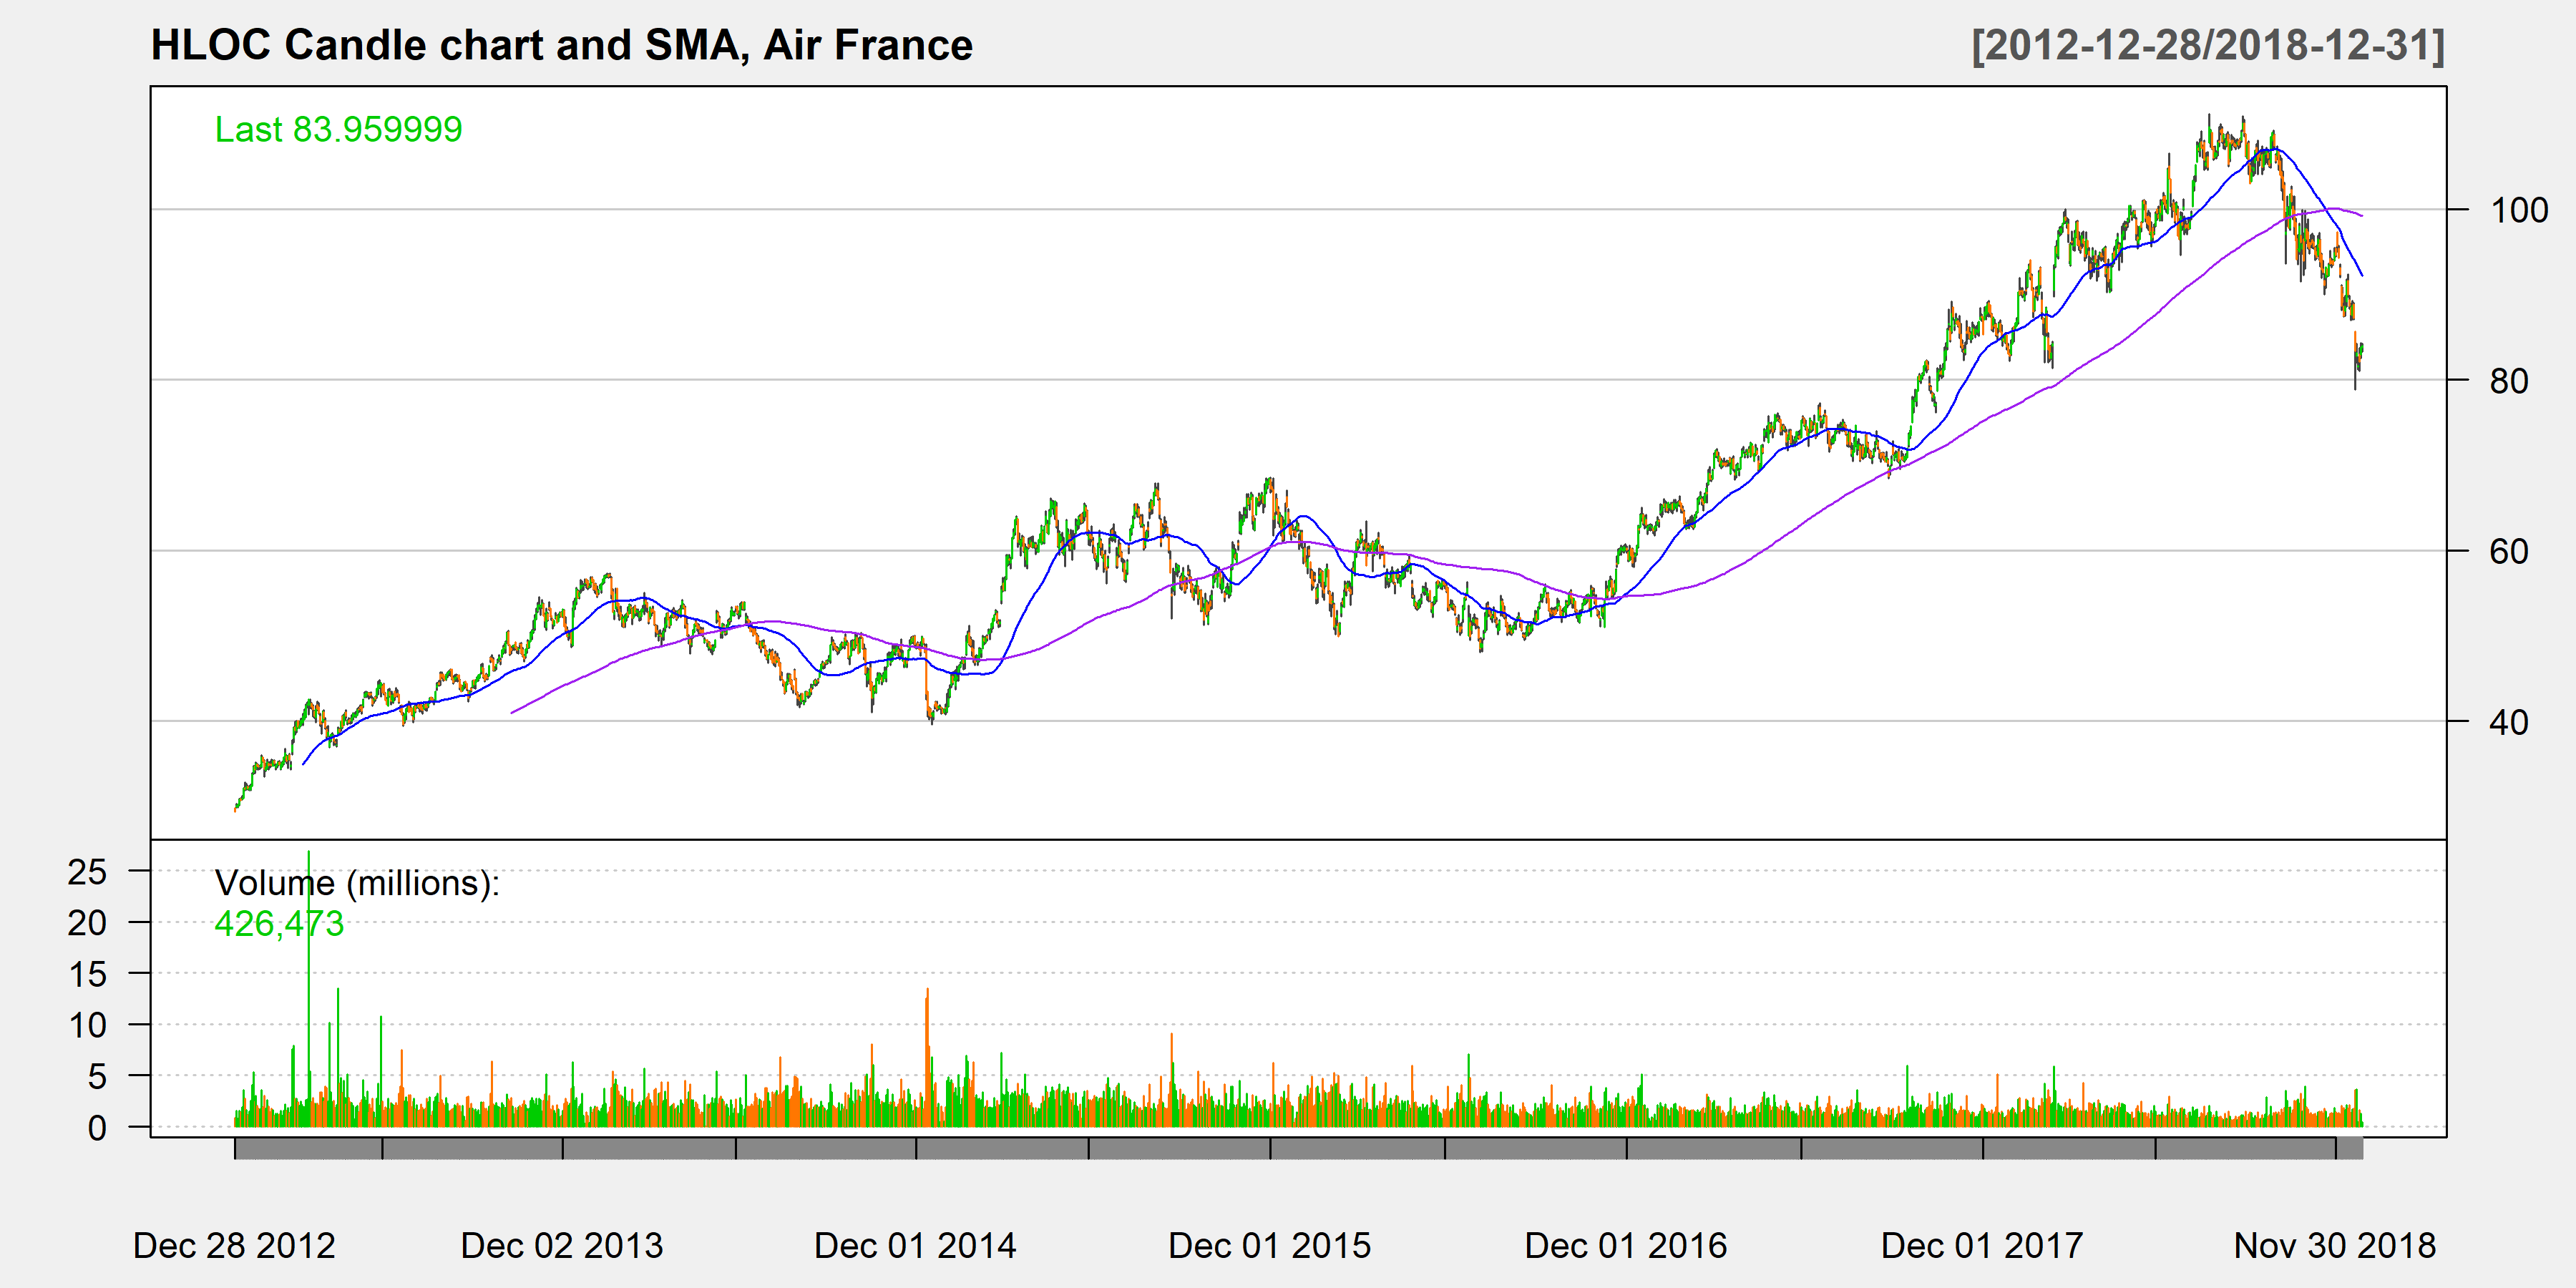
\includegraphics{"D:/2017-2018/data_analysis/technical_analysis/report/HLOC Candle chart and SMA, Air France.png"}
\caption{Daily HLOC Chart price, with SMA(50) in blu, and SMA(200) in
purple.}
\end{figure}

The SMA is used to smooth out the price trends from the short-term
fluctations. Usually, (at least) two SMA's of different time-lags are
used together to generate trading signals. The short-term average
crossing from below the long-term average is considered a buy signal,
whereas a crossing in the other direction is taken as an indication to
sell. One common choice for the lags are the 50- and the 200-days
averages.

The second indicator is the \textbf{Relative Strength Index}, or RSI .
It is computed as\\
\begin{equation} 
RSI = 100 - \left( \frac{100}{(1 + \frac{\Delta_u}{\Delta_d} } \right) 
\end{equation} where \(\Delta_u =\) Average of Upward Price Change, and
\(\Delta_d =\) Average of Downward Price Change\footnote{\url{https://www.fidelity.com/learning-center/trading-investing/technical-analysis/technical-indicator-guide/RSI}}.
(See also \citet{Hsu2016} for an example of different parametrizations.)

The RSI is an oscillator, since its value is in the range {[}0,100{]}.
It gives indications on the \textbf{momentum}, that is, the ``the
magnitude of recent price changes to evaluate overbought or oversold
conditions in the price of a stock or other asset.''\footnote{\url{https://www.investopedia.com/terms/r/rsi.asp}}
Generally, \(RSI>70\) is taken as an indication for a security to be
overbought, whereas \(RSI < 30\) has the opposite meaning.

\begin{Shaded}
\begin{Highlighting}[]
\NormalTok{quantmod}\OperatorTok{::}\KeywordTok{addRSI}\NormalTok{(}\DataTypeTok{n=}\DecValTok{14}\NormalTok{, }\DataTypeTok{maType=} \StringTok{'SMA'}\NormalTok{) }
\CommentTok{# the RSI is shown, albeit not overimposed to the price pattern}
\end{Highlighting}
\end{Shaded}

\begin{figure}
\centering
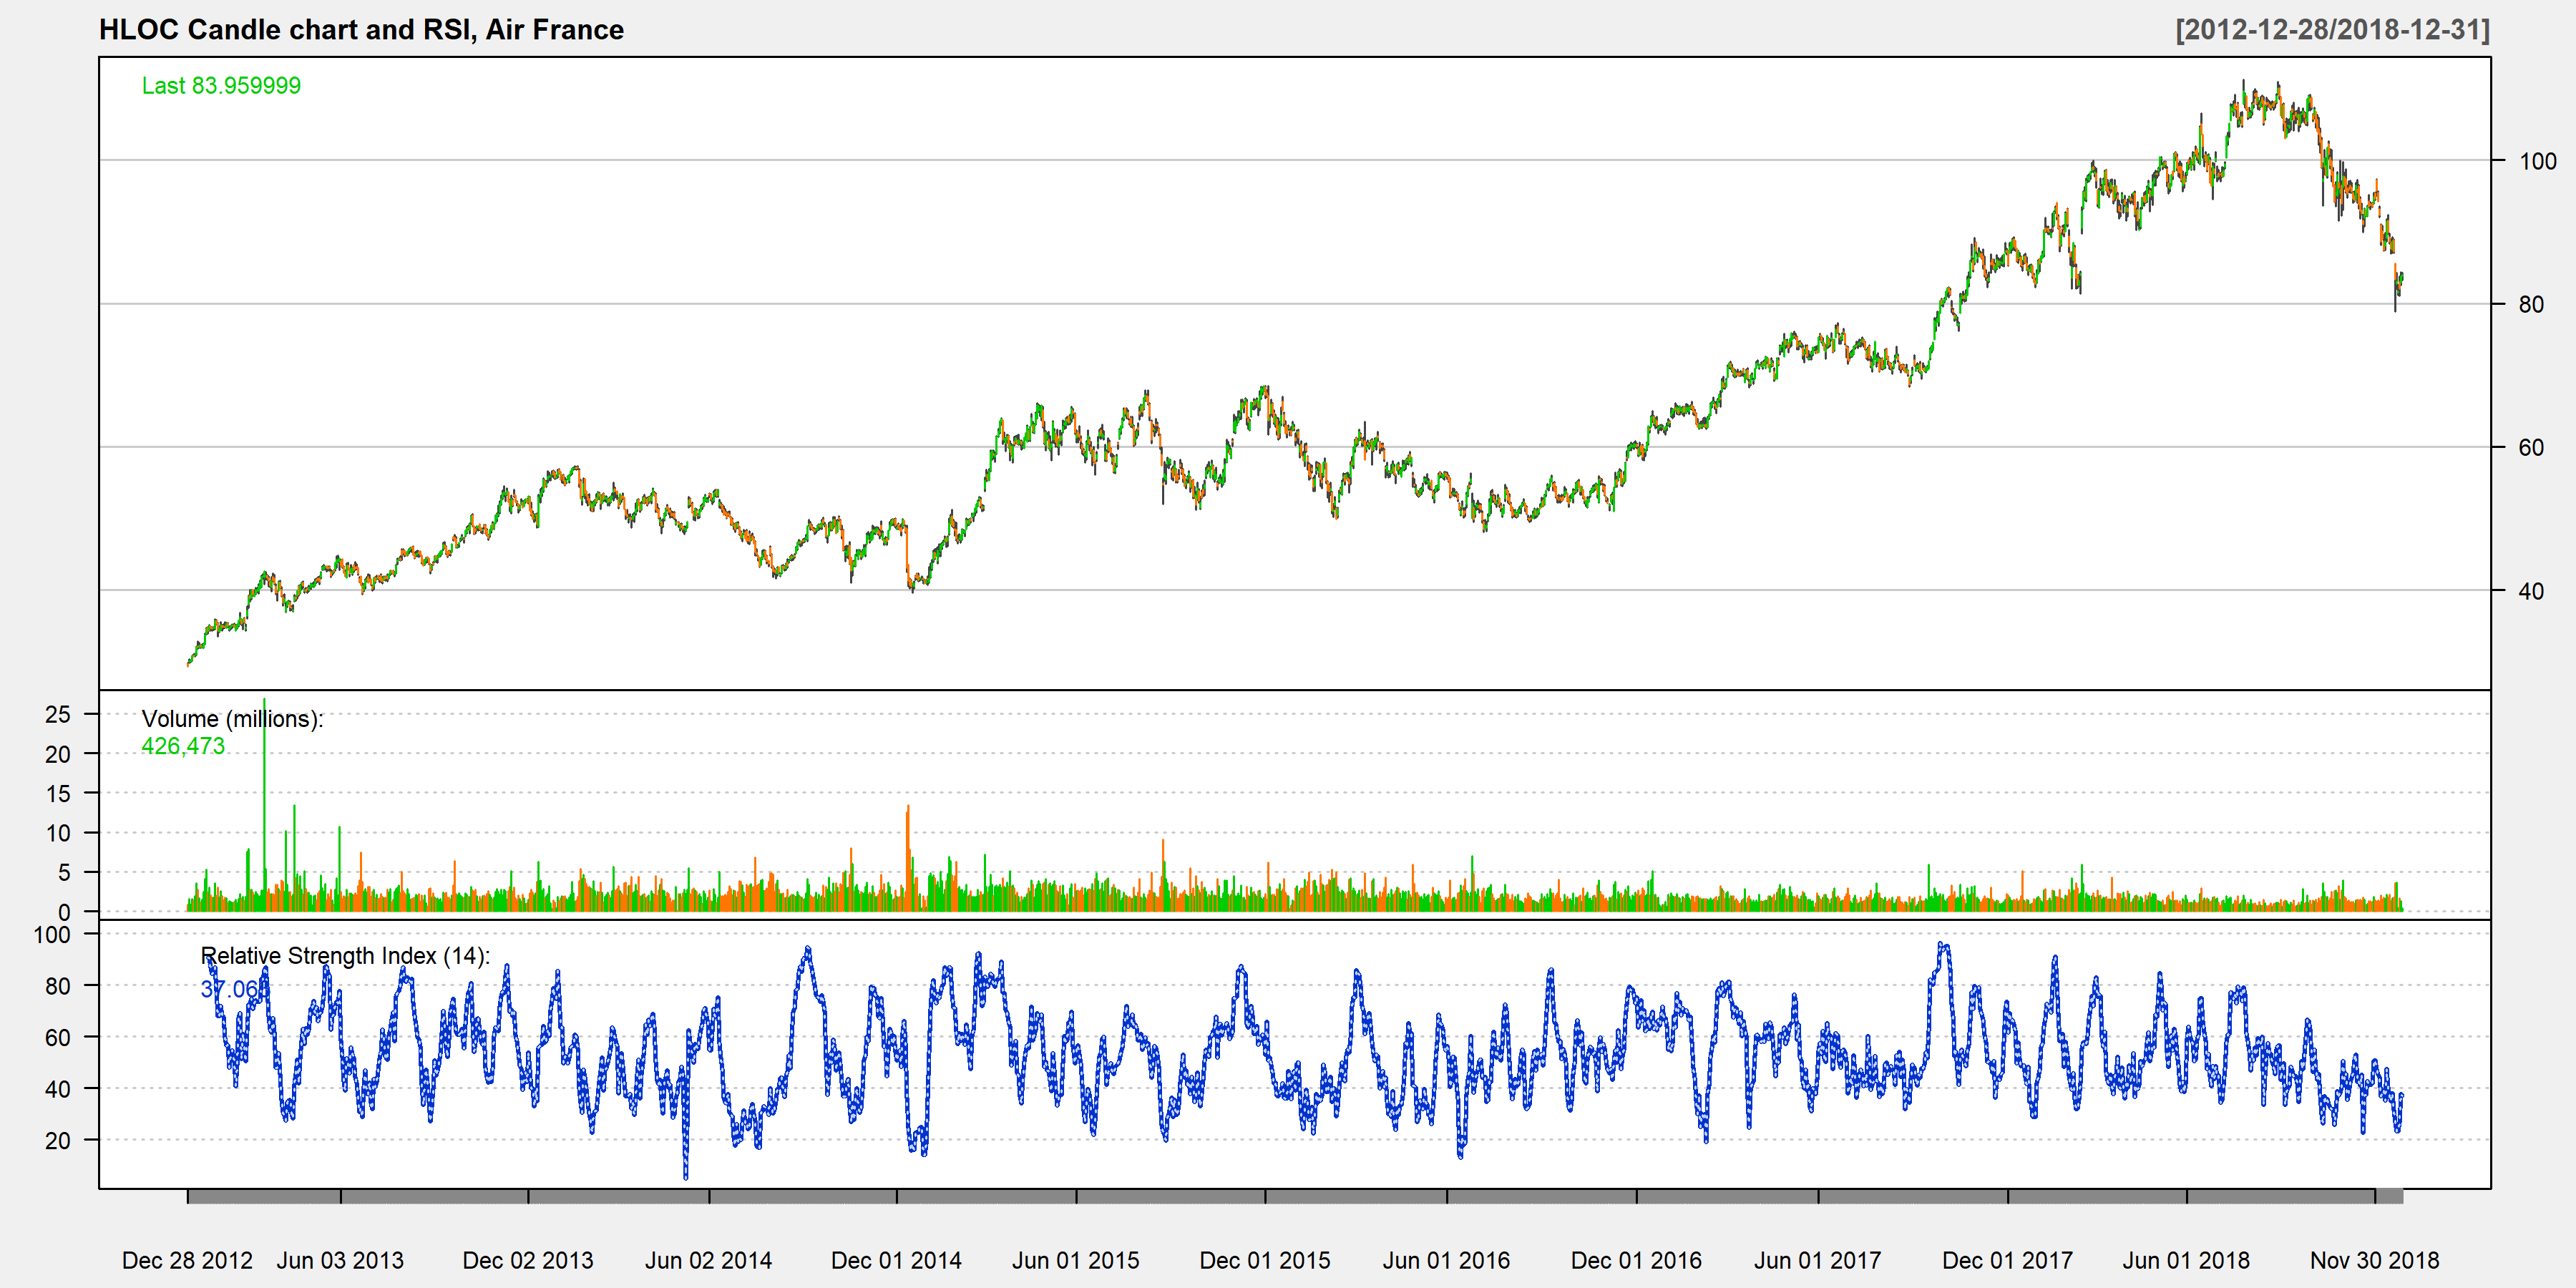
\includegraphics{"D:/2017-2018/data_analysis/technical_analysis/report/HLOC Candle chart and RSI, Air France.png"}
\caption{Daily HLOC Chart price with RSI(14)}
\end{figure}

The third indicator are the \textbf{Bollinger Bands} \footnote{\url{https://www.bollingerbands.com/}}.
These are defined by the plot of a simple moving average, as defined
below by the \(\mu\), along with its standard deviation around it,
defining the upper and lower bands. These are defined respectively as
\begin{equation}
B_u = MA(\mu, n) + m \cdot \sigma(\mu,n)
\end{equation} and \begin{equation}
B_d = MA(\mu, n) - m \cdot \sigma(\mu,n)
\end{equation}

with

\(HLC_t:=High_t +Low_t + Close_t\);

\(\mu= \frac{HLC_t}{3}\);

\(\sigma_n= \sqrt{\displaystyle \frac{\sum_{t=1}^{n} {(HLC_t-\mu)^2}}{n}}\)
the standard deviation of HLC over n days;

\(n \in \mathbb{N^*}\) the number of days over which the SMA is
computed;

\(m \in \mathbb{N^*}\) the number of standard deviations used to create
the width of the bands.

A common parametrization of this indicator is one with
two-standard-deviation-wide bands around a 20-day simple moving average
(i.e.~\(m=2\),\(n=20\)).

\begin{Shaded}
\begin{Highlighting}[]
\KeywordTok{addBBands}\NormalTok{(}\DataTypeTok{n=}\DecValTok{20}\NormalTok{, }\DataTypeTok{sd=}\DecValTok{2}\NormalTok{, }\DataTypeTok{maType=} \StringTok{"SMA"}\NormalTok{) }
\end{Highlighting}
\end{Shaded}

\begin{figure}
\centering
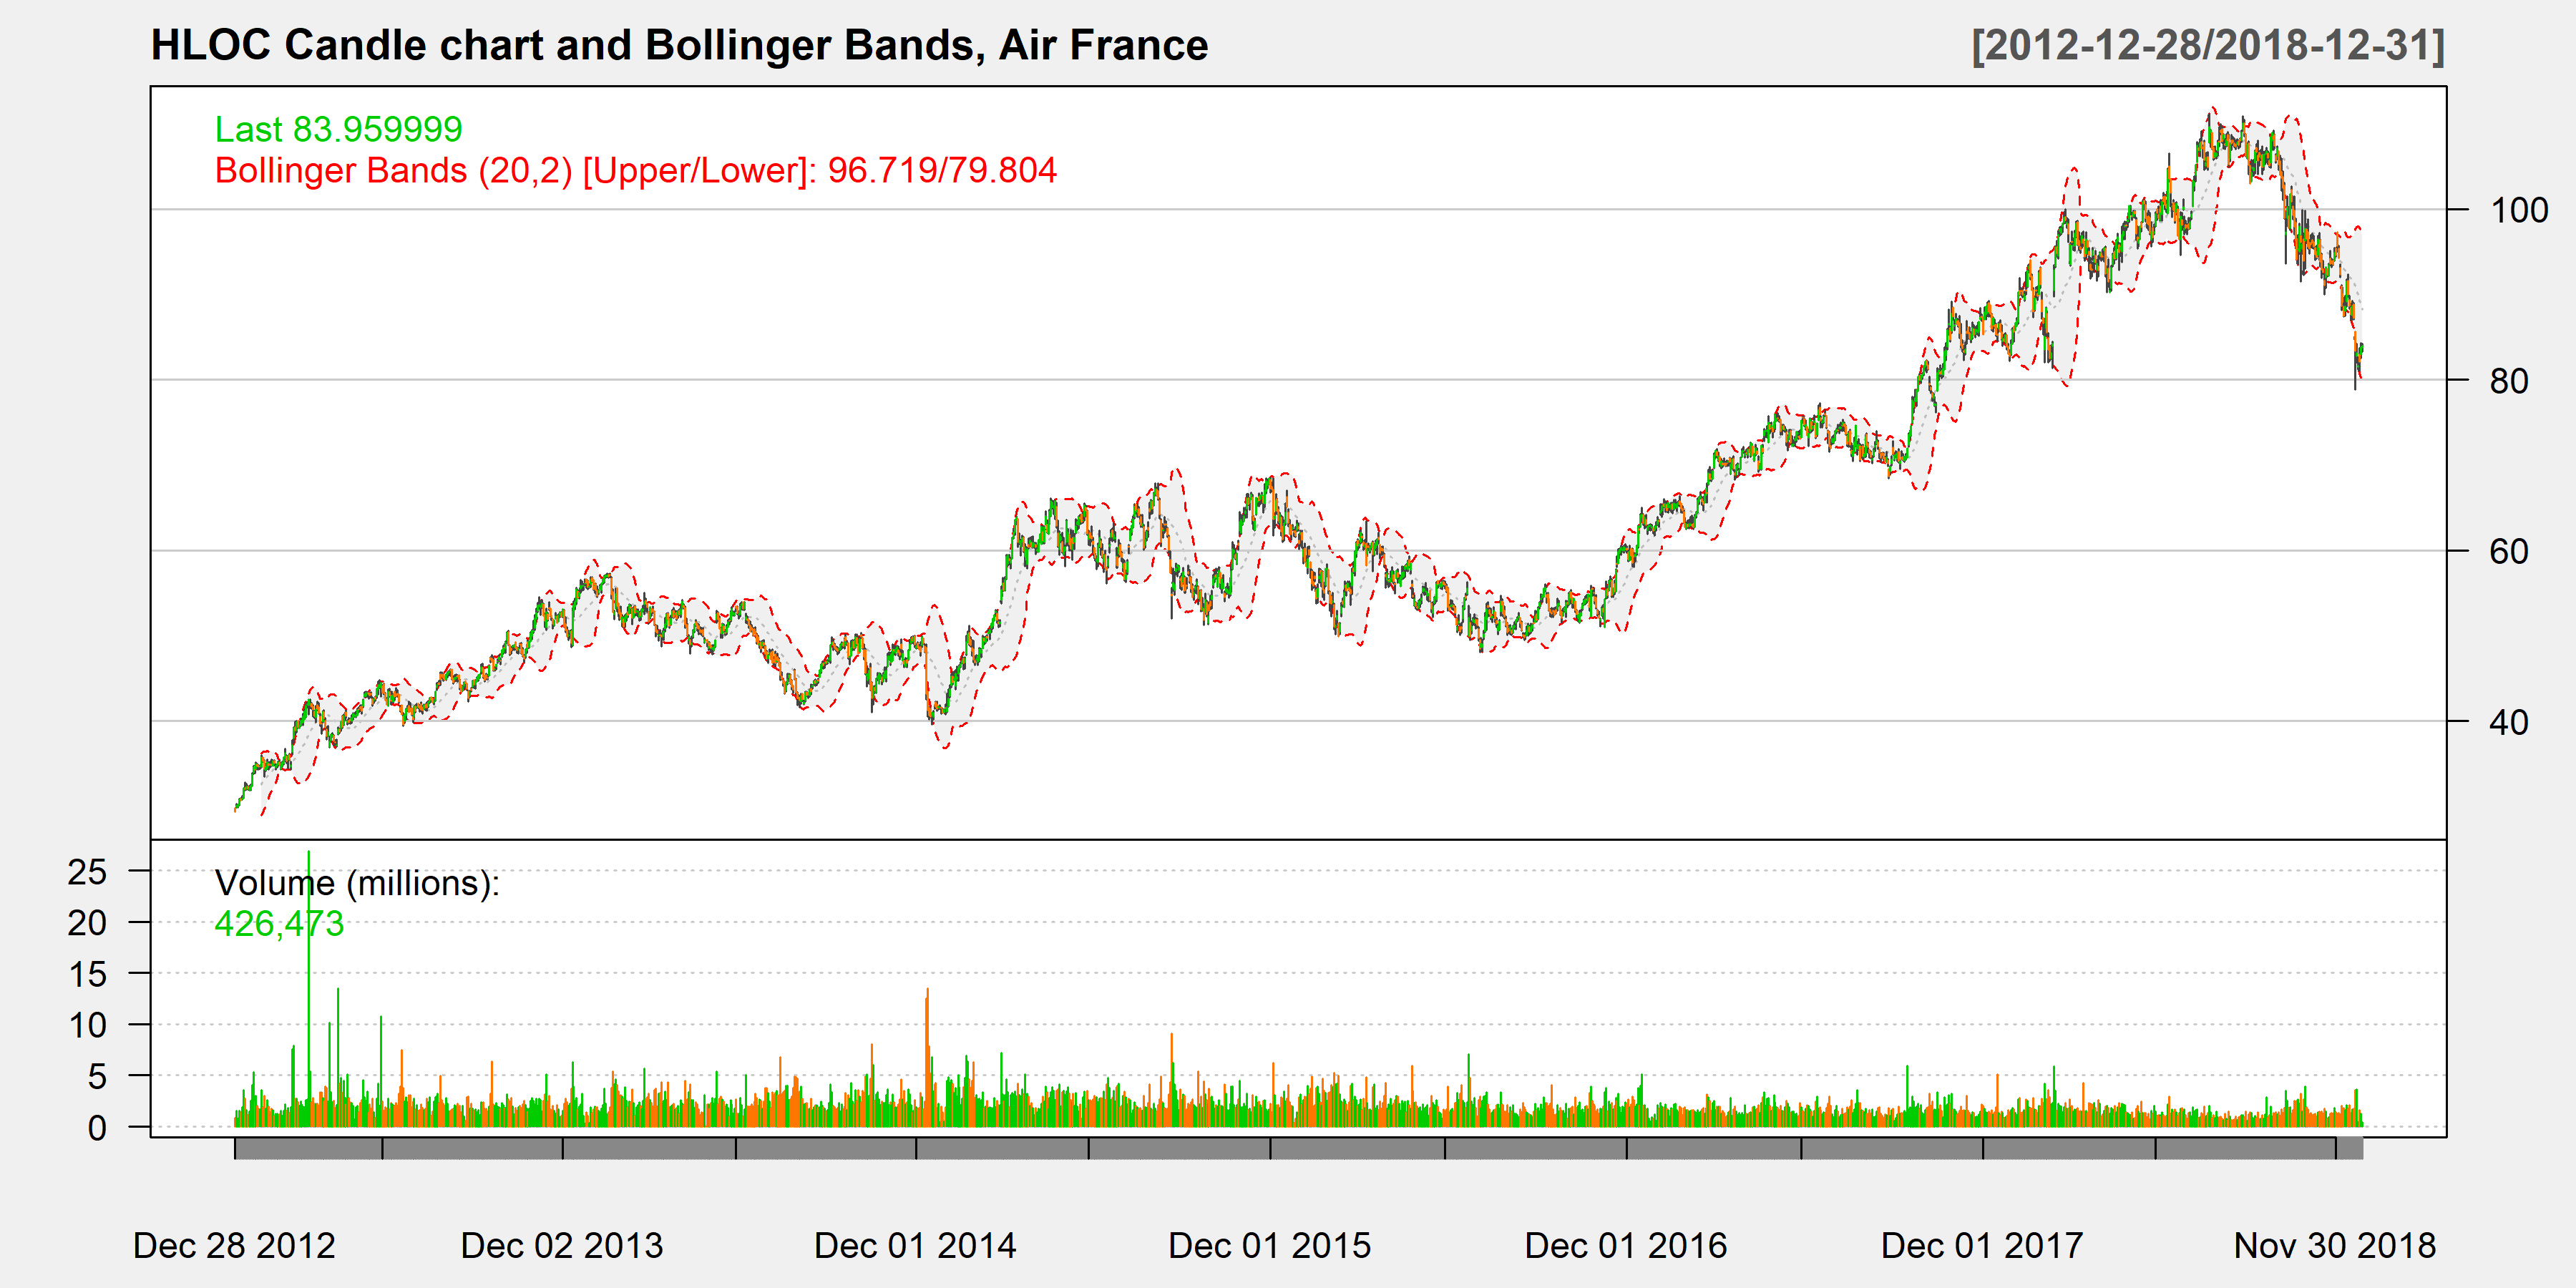
\includegraphics{"D:/2017-2018/data_analysis/technical_analysis/report/HLOC Candle chart and Bollinger Bands, Air France.png"}
\caption{Daily HLOC Chart price with Bollinger Bands (20,2)}
\end{figure}

\hypertarget{quantmod-blotter-and-quantstrat-packages}{%
\subsection{quantmod, blotter and quantstrat
packages}\label{quantmod-blotter-and-quantstrat-packages}}

One important building block towards the implementation of Technical
Analysis in R is the package quantmod\footnote{\url{https://github.com/joshuaulrich/quantmod}},
which allows the user to download stock prices data from Yahoo! Finance,
and to visualize different types of price charts, which are of great
support in a first, rough analysis of the evolution of price trends over
time. For the sake of offering a visual understanding of TA indicators,
these functionalities were already exploited in the previuous paragraph,
using the functions \texttt{quantmod::getSymbols()} and
\texttt{quantmod::chartSeries}, along with \texttt{quantmod::addSMA},
\texttt{quantmod::addRSI}, and \texttt{quantmod::addBBands}.

Moreover, R supports a package named \texttt{quantstrat}, a
``transaction-oriented infrastructure for constructing trading systems
and simulation\footnote{\url{https://www.rdocumentation.org/packages/quantstrat/versions/0.16.6}}''.
However, this package counts several dependencies, and therefore we'll
need our machine to be equipped with all these packages, as brilliantly
shown in \citet{Yu2019}.

\begin{Shaded}
\begin{Highlighting}[]
\KeywordTok{install.packages}\NormalTok{(}\StringTok{"quantmod"}\NormalTok{)}
\KeywordTok{install.packages}\NormalTok{(}\StringTok{"FinancialInstrument"}\NormalTok{)}
\KeywordTok{install.packages}\NormalTok{(}\StringTok{"PerformanceAnalytics"}\NormalTok{)}
\KeywordTok{install.packages}\NormalTok{(}\StringTok{"foreach"}\NormalTok{)}
\KeywordTok{install.packages}\NormalTok{(}\StringTok{"devtools"}\NormalTok{)}
\NormalTok{devtools}\OperatorTok{::}\KeywordTok{install_github}\NormalTok{(}\StringTok{"braverock/blotter"}\NormalTok{)}
\NormalTok{devtools}\OperatorTok{::}\KeywordTok{install_github}\NormalTok{(}\StringTok{"braverock/quanstrat"}\NormalTok{)}
\end{Highlighting}
\end{Shaded}

\hypertarget{portfolio-management-with-quantstrat}{%
\subsection{Portfolio management with
quantstrat}\label{portfolio-management-with-quantstrat}}

We build an actilvely managed portfolio made of five of the top ten
firms of the CAC40, as of September 2019\footnote{The full list here:
  \url{https://live.euronext.com/en/product/indices/FR0003500008-XPAR/market-information}},
using six years of data, from 2012-12-28 to 2018-12-31, for a total of
1534 trading days. We highlight that the choice of the stocks felt
simply on some of the most liquid Starting with an initial capital of €
100,000, we will buy or sell 100 stocks of each equity, whenever some
conditions on historic prices are met. These conditions are later
referred to as \emph{signals}, and are linked to the TA indicators
illustrated in their mathematical essence in the previuos part. We then
offer an overview on how to translate these mathematical conditions into
a `quantstrat' action in the sections that follow.

\begin{table}[ht]
\caption:{Top ten firms in CAC40 by market cap, September 2019}
\centering
\begin{tabular}{|c|c|c|c|}
  \hline
Company & MNEMO  &  Sector  & Weight\% \\
  \hline
  TOTAL &   FP  & Oil and Gas & 9,54 \\
  LVMH &    MC  & Personal and Household Goods & 7,97 \\
  SANOFI & SAN  & Health Care & 7,54 \\
  AIRBUS & AIR  & Industrial Goods and Services &   5,47 \\
  L'OREAL   & OR  & Personal and Household Goods &  5,10 \\
  AIR LIQUIDE & AI  & Chemicals &   4,40 \\
  DANONE &  BN  & Food and Beverage & 4,14 \\
  VINCI &   DG & Construction and Materials & 3,97 \\
  BNP PARIBAS ACT.A &   BNP  & Banks & 3,95 \\
  SAFRAN & SAF  & Industrial Goods and Services & 3,72 \\
   \hline
\end{tabular}
\end{table}

\hypertarget{preliminary-setup}{%
\subsubsection{Preliminary setup}\label{preliminary-setup}}

We first retrieve data from Yahoo to the R global environment:

\begin{Shaded}
\begin{Highlighting}[]
\NormalTok{from =}\StringTok{"2012-12-28"}
\NormalTok{to =}\StringTok{"2018-12-31"}
\NormalTok{symbols =}\StringTok{ }\KeywordTok{c}\NormalTok{(}\StringTok{"MC.PA"}\NormalTok{,}\StringTok{"BN.PA"}\NormalTok{,}\StringTok{"AIR.PA"}\NormalTok{,}\StringTok{"BNP.PA"}\NormalTok{,}\StringTok{"DG.PA"}\NormalTok{ )}
\CommentTok{# the .PA label is needed to specify the Paris CAC40 stock exchange}
\NormalTok{quantmod}\OperatorTok{::}\KeywordTok{getSymbols}\NormalTok{(symbols,}
                     \DataTypeTok{from=}\NormalTok{from, }\DataTypeTok{to=}\NormalTok{to)}
\end{Highlighting}
\end{Shaded}

We then set up the strategy, the portfolio and the account objects:

\begin{Shaded}
\begin{Highlighting}[]
\NormalTok{initEq=}\DecValTok{100000} \CommentTok{# capital to invest}

\NormalTok{strategy.st <-}\StringTok{ "strat.full.limit"} \CommentTok{# name the objects}
\NormalTok{portfolio.st <-}\StringTok{ "portf.full.limit"}
\NormalTok{account.st <-}\StringTok{ "acct.full.limit"}

\NormalTok{blotter}\OperatorTok{::}\KeywordTok{initPortf}\NormalTok{(portfolio.st, symbols) }\CommentTok{#initialize portfolio}
\NormalTok{blotter}\OperatorTok{::}\KeywordTok{initAcct}\NormalTok{(account.st, }\CommentTok{# also need specifing linked portfolio }
         \DataTypeTok{portfolios=}\NormalTok{portfolio.st, }
         \DataTypeTok{initEq =}\NormalTok{ initEq) }
\NormalTok{quantstrat}\OperatorTok{::}\KeywordTok{initOrders}\NormalTok{(portfolio.st) }\CommentTok{# the orders 'container'}
\NormalTok{quantstrat}\OperatorTok{::}\KeywordTok{strategy}\NormalTok{(strategy.st, }\DataTypeTok{store=}\OtherTok{TRUE}\NormalTok{) }\CommentTok{# we save our strategy in }
\CommentTok{# the global environement}
\end{Highlighting}
\end{Shaded}

\hypertarget{create-indicators}{%
\subsubsection{Create indicators}\label{create-indicators}}

As illustrated earlier, we make use of three simple indicators: simple
moving average, relative strength index and Bollinger Bands. The
indicators will be linked to the startegy object previoulsy defined. The
input dataframe is called \emph{mktdata}, an object that will be created
authomatically when we validate the strategy.

\begin{Shaded}
\begin{Highlighting}[]
\NormalTok{quantstrat}\OperatorTok{::}\KeywordTok{add.indicator}\NormalTok{(}
\NormalTok{  strategy.st, }\DataTypeTok{name=}\StringTok{"SMA"}\NormalTok{, }\CommentTok{# "name" must correspond to an R function}
  \DataTypeTok{arguments=} \KeywordTok{list}\NormalTok{(}\DataTypeTok{x=} \KeywordTok{quote}\NormalTok{(}\KeywordTok{Cl}\NormalTok{(mktdata)), }\DataTypeTok{n=}\DecValTok{50}\NormalTok{), }\CommentTok{# input data are closing prices}
  \CommentTok{# set input data (mktdata) and indicator parameters through function 'arguments'}
  \DataTypeTok{label=}\StringTok{"sma50"}\NormalTok{) }\CommentTok{## unique reference 'mktdata' column name}

\KeywordTok{add.indicator}\NormalTok{(}\DataTypeTok{strategy =}\NormalTok{ strategy.st,}
              \DataTypeTok{name =} \StringTok{'RSI'}\NormalTok{, }\CommentTok{# normally, we'll be using functions }
              \CommentTok{# from the TTR package }
              \DataTypeTok{arguments =} \KeywordTok{list}\NormalTok{(}\DataTypeTok{price =} \KeywordTok{quote}\NormalTok{(}\KeywordTok{Cl}\NormalTok{(mktdata)), }\DataTypeTok{n=}\DecValTok{14}\NormalTok{), }
              \CommentTok{# among the 'arguments', we need to set the }
              \CommentTok{# parameter (number of days of the SMA) for the RSI}
              \DataTypeTok{label =} \StringTok{'rsi.14'}\NormalTok{)}

\KeywordTok{add.indicator}\NormalTok{(}\DataTypeTok{strategy =}\NormalTok{ strategy.st,}
              \DataTypeTok{name=} \StringTok{"BBands"}\NormalTok{, }
              \DataTypeTok{arguments =} 
                \KeywordTok{list}\NormalTok{(}\DataTypeTok{HLC =} \KeywordTok{quote}\NormalTok{(}\KeywordTok{HLC}\NormalTok{(mktdata)),}\DataTypeTok{n=}\DecValTok{20}\NormalTok{, }\DataTypeTok{maType=} \StringTok{"SMA"}\NormalTok{, }\DataTypeTok{sd=}\DecValTok{2}\NormalTok{), }
              \CommentTok{# BBands need High,Low and Closing Prices as an Input}
              \DataTypeTok{label =} \StringTok{"bb.20.2"}\NormalTok{)}
\end{Highlighting}
\end{Shaded}

\hypertarget{combining-indicators-to-create-trading-signals}{%
\subsubsection{Combining indicators to create trading
signals}\label{combining-indicators-to-create-trading-signals}}

The third step after setting up the blotter objects and creating the
indicators, is creating buy and sell signals out of an appropriate blend
of indicators. Below we offer a summary of the signals that will be used
here.

\begin{table}[ht]
\caption{Summary of signals and related trading executions}
\centering
\begin{tabular}{|c|c|c|c|}
  \hline
Type of Signal (quantmod) & Signal & Execution & Label \\ 
  \hline
  Crossover & SMA(50)>SMA(200) & NA & smabuy \\ 
  Crossover & SMA(50)<SMA(200) & NA & smasell \\ 
  Threshold & RSI<30  & NA & rsi14buy\\ 
  Threshold & RSI>70  & NA & rsi14sell \\ 
  Crossover & Closing > Upper BBand  & NA & Cl.gt.UpperBand \\ 
  Crossover & Closing < Lower BBand  & NA & Cl.lt.LowerBand \\ 
  Crossover and Threshold & SMA(50)>SMA(200) and RSI<30 & Buy & entry1 \\ 
  Crossover and Threshold & SMA(50)<SMA(200) and RSI>70 & Sell & exit1 \\ 
  Crossover and Threshold & Closing < Lower BBand and RSI<30 & Buy & entry2 \\
  Crossover and Threshold & Closing > Upper BBand and RSI>70 & Sell & exit2 \\
   \hline
\end{tabular}
\end{table}

Despite having defined ten signals, only four of these will trigger
actual execution orders. This is because it looks safer to rely on a
mixed signal - i.e.~one making use of more than one indicator - rather
than only on a simple one.

Here is some code showing how a mixed signal is created, based on the
evaluation of two simple ones, which in turn may have different level of
complexities, depending on the kind of indicators used to build them.
Notice that the function \texttt{sigFormula} can take more than two
arguments, evaluating therefore several conditions at once.

\begin{Shaded}
\begin{Highlighting}[]
\CommentTok{## 'Bull market' (i.e. market considered underpriced --> indication to buy) }
\CommentTok{# if SMA50>SMA200}
\NormalTok{quantstrat}\OperatorTok{::}\KeywordTok{add.signal}\NormalTok{(}
\NormalTok{  strategy.st, }\DataTypeTok{name=}\StringTok{"sigCrossover"}\NormalTok{, }\CommentTok{## "name" is a function taking on}
           \CommentTok{# specific arguments }
           \DataTypeTok{arguments=} \KeywordTok{list}\NormalTok{(}\DataTypeTok{columns=}\KeywordTok{c}\NormalTok{(}\StringTok{"sma50"}\NormalTok{,}\StringTok{"sma200"}\NormalTok{),}\DataTypeTok{relationship=}\StringTok{"gt"}\NormalTok{), }
            \CommentTok{# 'columns' refers to the indicators defined above}
           \DataTypeTok{label=}\StringTok{"smabuy"}\NormalTok{) }\CommentTok{# 'label' will be the reference for }
\CommentTok{# the execution phase hereafter.}

\CommentTok{## Specifies all instance when RSI is below 30 }
\CommentTok{## (indication of asset being oversold)}
\KeywordTok{add.signal}\NormalTok{(strategy.st, }\DataTypeTok{name =} \StringTok{"sigThreshold"}\NormalTok{,}
           \DataTypeTok{arguments =} 
             \KeywordTok{list}\NormalTok{(}\DataTypeTok{column =} \StringTok{"rsi.14"}\NormalTok{, }\DataTypeTok{threshold =} \DecValTok{30}\NormalTok{, }\DataTypeTok{relationship =} \StringTok{"lt"}\NormalTok{, }
                  \DataTypeTok{cross =} \OtherTok{TRUE}\NormalTok{), }\CommentTok{# signals }
           \DataTypeTok{label =} \StringTok{"rsi14buy"}\NormalTok{)}

\CommentTok{## sigFormula which indicates that both smabuy and rsi14buy must evaluate TRUE.}
\KeywordTok{add.signal}\NormalTok{(strategy.st, }\DataTypeTok{name =} \StringTok{"sigFormula"}\NormalTok{,}
           \DataTypeTok{arguments =} \KeywordTok{list}\NormalTok{(}\DataTypeTok{formula =} \StringTok{"smabuy & rsi14buy"}\NormalTok{,}\DataTypeTok{cross =} \OtherTok{TRUE}\NormalTok{),}
           \CommentTok{# notice that the formula is evaluating two booleans }
           \DataTypeTok{label =} \StringTok{"entry1"}\NormalTok{) }
\end{Highlighting}
\end{Shaded}

\hypertarget{executing-tradings}{%
\subsubsection{Executing tradings}\label{executing-tradings}}

The very last step of our strategy will be defining the trading
operations to execute, once the relevant signals are observed. As shown
in the table above, only four signals trigger an order execution. We
define accordingly four trading execution rules.

\begin{Shaded}
\begin{Highlighting}[]
\CommentTok{## Enter the position when SMA(50)>SMA(200), and the RSI<30}
\NormalTok{quantstrat}\OperatorTok{::}\KeywordTok{add.rule}\NormalTok{(}
\NormalTok{  strategy.st, }\DataTypeTok{name =} \StringTok{"ruleSignal"}\NormalTok{,}
         \DataTypeTok{arguments =} \KeywordTok{list}\NormalTok{(}\DataTypeTok{sigcol =} \StringTok{"entry1"}\NormalTok{, }\DataTypeTok{sigval =} \OtherTok{TRUE}\NormalTok{,}
                          \DataTypeTok{orderqty =} \DecValTok{1000}\NormalTok{, }\DataTypeTok{ordertype =} \StringTok{"market"}\NormalTok{,}
                          \DataTypeTok{orderside =} \StringTok{"long"}\NormalTok{, }\DataTypeTok{replace =} \OtherTok{FALSE}\NormalTok{,}
                          \DataTypeTok{prefer =} \StringTok{"Open"}\NormalTok{, }
                          \DataTypeTok{tradeSize =}\NormalTok{ tradesize, }\DataTypeTok{maxSize =}\NormalTok{ tradesize),}
         \DataTypeTok{type =} \StringTok{"enter"}\NormalTok{)  }


\CommentTok{## Exit the position when SMA(50)<SMA(200), and the RSI>70}
\KeywordTok{add.rule}\NormalTok{(strategy.st, }\DataTypeTok{name =} \StringTok{"ruleSignal"}\NormalTok{,}
         \DataTypeTok{arguments =} \KeywordTok{list}\NormalTok{(}\DataTypeTok{sigcol =} \StringTok{"exit1"}\NormalTok{, }\DataTypeTok{sigval =} \OtherTok{TRUE}\NormalTok{,}
                          \DataTypeTok{orderqty =} \DecValTok{-1000}\NormalTok{ , }\DataTypeTok{ordertype =} \StringTok{"market"}\NormalTok{,}
                          \DataTypeTok{orderside =} \StringTok{"long"}\NormalTok{, }\DataTypeTok{replace =} \OtherTok{FALSE}\NormalTok{,}
                          \DataTypeTok{prefer =} \StringTok{"Open"}\NormalTok{, }
                          \DataTypeTok{tradeSize =}\NormalTok{ tradesize, }
                          \DataTypeTok{maxSize =}\NormalTok{ tradesize),}
         \DataTypeTok{type =} \StringTok{"exit"}\NormalTok{) }


\CommentTok{## Enter the position when (Closing price < Lower BBand) and RSI<30}
\KeywordTok{add.rule}\NormalTok{(}\DataTypeTok{strategy =}\NormalTok{ strategy.st, }\DataTypeTok{name=} \StringTok{'ruleSignal'}\NormalTok{,}
         \DataTypeTok{arguments =} \KeywordTok{list}\NormalTok{(}\DataTypeTok{sigcol =} \StringTok{"entry2"}\NormalTok{, }\DataTypeTok{sigval=} \OtherTok{TRUE}\NormalTok{,}
                          \DataTypeTok{orderqty =} \DecValTok{1000}\NormalTok{, }\DataTypeTok{ordertype=} \StringTok{'market'}\NormalTok{, }
                          \DataTypeTok{orderside=} \OtherTok{NULL}\NormalTok{,}\DataTypeTok{threshold=}\OtherTok{NULL}\NormalTok{ ), }
         \DataTypeTok{type=} \StringTok{"enter"}\NormalTok{)}


\CommentTok{## Exit the position when (Closing price > Upper BBand) and RSI>70  }
\KeywordTok{add.rule}\NormalTok{(}\DataTypeTok{strategy =}\NormalTok{ strategy.st, }\DataTypeTok{name=} \StringTok{'ruleSignal'}\NormalTok{,}
         \DataTypeTok{arguments =} \KeywordTok{list}\NormalTok{(}\DataTypeTok{sigcol =} \StringTok{"exit2"}\NormalTok{, }\DataTypeTok{sigval=} \OtherTok{TRUE}\NormalTok{,}
                          \DataTypeTok{orderqty =} \DecValTok{-1000}\NormalTok{, }\DataTypeTok{ordertype=} \StringTok{'market'}\NormalTok{, }\DataTypeTok{orderside=} \OtherTok{NULL}\NormalTok{,}
                          \DataTypeTok{threshold=}\OtherTok{NULL}\NormalTok{ ),  }
         \DataTypeTok{type=} \StringTok{"exit"}\NormalTok{)}
\end{Highlighting}
\end{Shaded}

\hypertarget{running-the-model}{%
\subsubsection{Running the model}\label{running-the-model}}

At this stage, we are ready to run our model. It is safer to check first
whether the code for the strategy we seek to implement is `bug-free'. To
do this, we run the \texttt{quantstrat::applyStrategy} command within
the \texttt{base::try} function, which allows to ``run an expression
that might fail and allow the user's code to handle
error-recovery''\footnote{\url{https://stat.ethz.ch/R-manual/R-devel/library/base/html/try.html}}.

\begin{Shaded}
\begin{Highlighting}[]
\NormalTok{testing_strat <-}\StringTok{ }\NormalTok{base}\OperatorTok{::}\KeywordTok{try}\NormalTok{( quantstrat}\OperatorTok{::}\KeywordTok{applyStrategy}\NormalTok{(strategy.st,}
                        \DataTypeTok{portfolios=}\NormalTok{portfolio.st ))}
\CommentTok{## try is a function in one of the basis R packages}

\CommentTok{## We test whether our entire startegy was coded correctly }
\end{Highlighting}
\end{Shaded}

\begin{verbatim}
## [1] "Set capital to 100,000 Euros "
## initalize portfolio: portf.fullinitalize account: acct.fullinitializie strategy: strat.full[1] "2013-02-20 00:00:00 AIR.PA -100 @ 36.25"
## [1] "2013-08-01 00:00:00 AIR.PA -100 @ 45.275002"
## [1] "2013-10-07 00:00:00 AIR.PA -100 @ 50.299999"
## [1] "2014-07-17 00:00:00 AIR.PA 100 @ 44.98"
## [1] "2014-09-05 00:00:00 AIR.PA -100 @ 49.189999"
## [1] "2015-01-26 00:00:00 AIR.PA -100 @ 50.139999"
## [1] "2015-02-19 00:00:00 AIR.PA -100 @ 51.990002"
## [1] "2015-03-02 00:00:00 AIR.PA -100 @ 56.09"
## [1] "2016-06-14 00:00:00 AIR.PA 100 @ 50.98"
## [1] "2016-06-17 00:00:00 AIR.PA 100 @ 50.830002"
## [1] "2016-12-14 00:00:00 AIR.PA -100 @ 62.400002"
## [1] "2016-12-16 00:00:00 AIR.PA -100 @ 64.18"
## [1] "2017-02-24 00:00:00 AIR.PA -100 @ 68.349998"
## [1] "2017-10-25 00:00:00 AIR.PA -100 @ 83.470001"
## [1] "2017-11-01 00:00:00 AIR.PA -100 @ 87.379997"
## [1] "2018-06-15 00:00:00 AIR.PA -100 @ 103.599998"
## [1] "2013-06-25 00:00:00 FP.PA 100 @ 36.294998"
## [1] "2013-08-26 00:00:00 FP.PA -100 @ 42"
## [1] "2013-08-29 00:00:00 FP.PA -100 @ 42.509998"
## [1] "2014-05-09 00:00:00 FP.PA -100 @ 52.259998"
## [1] "2014-10-16 00:00:00 FP.PA 100 @ 42.555"
## [1] "2017-07-10 00:00:00 FP.PA 100 @ 42.764999"
## [1] "2018-05-18 00:00:00 FP.PA -100 @ 54.48"
## [1] "2014-01-09 00:00:00 MC.PA 100 @ 122.949997"
## [1] "2014-04-11 00:00:00 MC.PA -100 @ 141.199997"
## [1] "2014-07-28 00:00:00 MC.PA 100 @ 131.550003"
## [1] "2014-11-24 00:00:00 MC.PA -100 @ 144.300003"
## [1] "2014-12-18 00:00:00 MC.PA 100 @ 130.25"
## [1] "2015-02-05 00:00:00 MC.PA -100 @ 153.5"
## [1] "2015-03-12 00:00:00 MC.PA -100 @ 170.600006"
## [1] "2016-07-28 00:00:00 MC.PA -100 @ 153.350006"
## [1] "2016-10-12 00:00:00 MC.PA -100 @ 164.350006"
## [1] "2016-10-17 00:00:00 MC.PA -100 @ 165.399994"
## [1] "2017-01-20 00:00:00 MC.PA -100 @ 190.949997"
## [1] "2017-03-20 00:00:00 MC.PA -100 @ 200"
## [1] "2017-04-03 00:00:00 MC.PA -100 @ 204.050003"
## [1] "2017-04-25 00:00:00 MC.PA -100 @ 223.149994"
## [1] "2017-10-27 00:00:00 MC.PA -100 @ 253.949997"
## [1] "2018-04-11 00:00:00 MC.PA -100 @ 278.25"
## [1] "2018-10-11 00:00:00 MC.PA 100 @ 261.950012"
## [1] "2013-01-30 00:00:00 OR.PA -100 @ 113.550003"
## [1] "2013-04-03 00:00:00 OR.PA -100 @ 127.300003"
## [1] "2018-02-09 00:00:00 OR.PA 100 @ 172.350006"
## [1] "2018-10-11 00:00:00 OR.PA 100 @ 187.600006"
## [1] "2013-04-03 00:00:00 SAN.PA -100 @ 80.050003"
## [1] "2013-11-07 00:00:00 SAN.PA -100 @ 78.660004"
## [1] "2014-10-16 00:00:00 SAN.PA 100 @ 78.800003"
## [1] "2014-10-29 00:00:00 SAN.PA 100 @ 71.150002"
## [1] "2015-02-16 00:00:00 SAN.PA -100 @ 85.720001"
## [1] "2015-02-20 00:00:00 SAN.PA -100 @ 87.389999"
## [1] "2015-02-24 00:00:00 SAN.PA -100 @ 88.75"
## [1] "2015-04-10 00:00:00 SAN.PA -100 @ 98.75"
## [1] "2016-06-15 00:00:00 SAN.PA 100 @ 68.110001"
## [1] "2016-11-10 00:00:00 SAN.PA -100 @ 76.980003"
## [1] "2017-04-05 00:00:00 SAN.PA -100 @ 85.43"
## [1] "2017-05-05 00:00:00 SAN.PA -100 @ 89.690002"
## [1] "2017-12-06 00:00:00 SAN.PA 100 @ 73.25"
## [1] "2018-07-05 00:00:00 SAN.PA -100 @ 72.440002"
## [1] "2018-08-01 00:00:00 SAN.PA -100 @ 75.599998"
\end{verbatim}

Since the strategy appears to run smoothly, we can update our portfolio
and account to register the transactions and variations in the level of
capital owned. We are now ready to extract the data on the performance,
in the form of summary statistics and charts. Unfortunately, it seems
that, due to an apparently still unfixed bug in the quantstrat
package\footnote{\url{https://github.com/braverock/quantstrat/issues/57}},
it is not possible to export the strategy log. This is why we kept it
printed to screen, as a full output of the command that runs the
relevant strategy implementation script.

\hypertarget{performance-evaluation}{%
\subsubsection{Performance evaluation}\label{performance-evaluation}}

As summarized in the first line of the table below, our strategy tested
on a five-year panel with five stocks seems `conservative', in that the
maximum number of tradings on a stock is 17 (for MC.PA), with an average
of roughly 12 across the five stocks. As the table below shows, for
three out of five stocks, the strategy net performance is negative. In
particular, trading on LVHM register a loss above €50,000. On the other
hand, the strategy yields a positive return for Total and Sanofi. The
lines ``Percent.Positive'' and ``Percent.Negative'', combined with
``Num.Trades'', gives an idea of how many open positions were closed
during the observed time frame, and if the operation carried a positive
or negative yield. By looking at the transaction log, one can see that
the strategy on both Air France was particualry unsuccessful because
several short positions were opened (hence, with the `expectation' of a
fall in the prices), and were (forcibly) closed only `at the end of the
world' i.e.~when we close the account and the portfolio at the end of
our observed period, after prices had rather steadly surged. For LVHM we
see a slightly different story, in which the first three couples of
operations are three profitable buy\&sell , after which the algorithms
becomes inefficient and determines the same patter as AIR.PA to be
observed. Sanofi looks like the example of a successful implementation
of our algorithm.

There are now some issues regarding our strategy that we would like to
higlight, and that would require further inspection and study:

\begin{itemize}
\item
  the first n days of observations (where n is the highest parameter
  value across all indicators making use of moving averages ) , should
  be left out. This is because during those n days only one out of two
  rules is implemented. This can clearly be source of biases. However,
  in this R framework , it does not seem possible to implement this
  option;
\item
  the algorithm parameters were set by a `thumb-rule' type of choice,
  i.e.~no action was taken to determine whether any further restrictons
  were to be put in place to obtain a better performance. For a better
  treatment on the code-related side of the matter, we refer the reader
  to \citet{Trice2016} for a reference to parameter optimization and
  backtesting ;
\item
  no in-depth study on the market conditions over the six years observed
  was made, neither on the specific stocks cases;
\item
  there is clearly the need for some constraints that prevent opening an
  excessive number of short positions - especially when the algorithm
  returns signals contrasting with price trend.
\end{itemize}

One caveat about the table that follows: it is generated through
\texttt{blotter::tradeStats}, and its output cannot be truncated.
Moreover, the function developement seems unfinished, as one can notice
from the uncomplete description of the statistics\footnote{Full account
  of the statistics here:
  \url{https://rdrr.io/rforge/blotter/man/tradeStats.html}} .

\begin{longtable}[]{@{}cccccc@{}}
\caption{Startegy trading statistics}\tabularnewline
\toprule
\begin{minipage}[b]{0.24\columnwidth}\centering
Measure\strut
\end{minipage} & \begin{minipage}[b]{0.10\columnwidth}\centering
AIR.PA\strut
\end{minipage} & \begin{minipage}[b]{0.10\columnwidth}\centering
FP.PA\strut
\end{minipage} & \begin{minipage}[b]{0.12\columnwidth}\centering
MC.PA\strut
\end{minipage} & \begin{minipage}[b]{0.10\columnwidth}\centering
OR.PA\strut
\end{minipage} & \begin{minipage}[b]{0.10\columnwidth}\centering
SAN.PA\strut
\end{minipage}\tabularnewline
\midrule
\endfirsthead
\toprule
\begin{minipage}[b]{0.24\columnwidth}\centering
Measure\strut
\end{minipage} & \begin{minipage}[b]{0.10\columnwidth}\centering
AIR.PA\strut
\end{minipage} & \begin{minipage}[b]{0.10\columnwidth}\centering
FP.PA\strut
\end{minipage} & \begin{minipage}[b]{0.12\columnwidth}\centering
MC.PA\strut
\end{minipage} & \begin{minipage}[b]{0.10\columnwidth}\centering
OR.PA\strut
\end{minipage} & \begin{minipage}[b]{0.10\columnwidth}\centering
SAN.PA\strut
\end{minipage}\tabularnewline
\midrule
\endhead
\begin{minipage}[t]{0.24\columnwidth}\centering
Num.Txns\strut
\end{minipage} & \begin{minipage}[t]{0.10\columnwidth}\centering
16\strut
\end{minipage} & \begin{minipage}[t]{0.10\columnwidth}\centering
7\strut
\end{minipage} & \begin{minipage}[t]{0.12\columnwidth}\centering
17\strut
\end{minipage} & \begin{minipage}[t]{0.10\columnwidth}\centering
4\strut
\end{minipage} & \begin{minipage}[t]{0.10\columnwidth}\centering
15\strut
\end{minipage}\tabularnewline
\begin{minipage}[t]{0.24\columnwidth}\centering
Num.Trades\strut
\end{minipage} & \begin{minipage}[t]{0.10\columnwidth}\centering
1\strut
\end{minipage} & \begin{minipage}[t]{0.10\columnwidth}\centering
3\strut
\end{minipage} & \begin{minipage}[t]{0.12\columnwidth}\centering
4\strut
\end{minipage} & \begin{minipage}[t]{0.10\columnwidth}\centering
1\strut
\end{minipage} & \begin{minipage}[t]{0.10\columnwidth}\centering
2\strut
\end{minipage}\tabularnewline
\begin{minipage}[t]{0.24\columnwidth}\centering
Net.Trading.PL\strut
\end{minipage} & \begin{minipage}[t]{0.10\columnwidth}\centering
-17778\strut
\end{minipage} & \begin{minipage}[t]{0.10\columnwidth}\centering
2346\strut
\end{minipage} & \begin{minipage}[t]{0.12\columnwidth}\centering
-52745\strut
\end{minipage} & \begin{minipage}[t]{0.10\columnwidth}\centering
-11910\strut
\end{minipage} & \begin{minipage}[t]{0.10\columnwidth}\centering
9853\strut
\end{minipage}\tabularnewline
\begin{minipage}[t]{0.24\columnwidth}\centering
Avg.Trade.PL\strut
\end{minipage} & \begin{minipage}[t]{0.10\columnwidth}\centering
-17778\strut
\end{minipage} & \begin{minipage}[t]{0.10\columnwidth}\centering
781.8\strut
\end{minipage} & \begin{minipage}[t]{0.12\columnwidth}\centering
-13186\strut
\end{minipage} & \begin{minipage}[t]{0.10\columnwidth}\centering
-11910\strut
\end{minipage} & \begin{minipage}[t]{0.10\columnwidth}\centering
4926\strut
\end{minipage}\tabularnewline
\begin{minipage}[t]{0.24\columnwidth}\centering
Med.Trade.PL\strut
\end{minipage} & \begin{minipage}[t]{0.10\columnwidth}\centering
-17778\strut
\end{minipage} & \begin{minipage}[t]{0.10\columnwidth}\centering
830\strut
\end{minipage} & \begin{minipage}[t]{0.12\columnwidth}\centering
1550\strut
\end{minipage} & \begin{minipage}[t]{0.10\columnwidth}\centering
-11910\strut
\end{minipage} & \begin{minipage}[t]{0.10\columnwidth}\centering
4926\strut
\end{minipage}\tabularnewline
\begin{minipage}[t]{0.24\columnwidth}\centering
Largest.Winner\strut
\end{minipage} & \begin{minipage}[t]{0.10\columnwidth}\centering
0\strut
\end{minipage} & \begin{minipage}[t]{0.10\columnwidth}\centering
570.5\strut
\end{minipage} & \begin{minipage}[t]{0.12\columnwidth}\centering
2325\strut
\end{minipage} & \begin{minipage}[t]{0.10\columnwidth}\centering
0\strut
\end{minipage} & \begin{minipage}[t]{0.10\columnwidth}\centering
2204\strut
\end{minipage}\tabularnewline
\begin{minipage}[t]{0.24\columnwidth}\centering
Largest.Loser\strut
\end{minipage} & \begin{minipage}[t]{0.10\columnwidth}\centering
-176.4\strut
\end{minipage} & \begin{minipage}[t]{0.10\columnwidth}\centering
0\strut
\end{minipage} & \begin{minipage}[t]{0.12\columnwidth}\centering
-6154\strut
\end{minipage} & \begin{minipage}[t]{0.10\columnwidth}\centering
-6718\strut
\end{minipage} & \begin{minipage}[t]{0.10\columnwidth}\centering
0\strut
\end{minipage}\tabularnewline
\begin{minipage}[t]{0.24\columnwidth}\centering
Gross.Profits\strut
\end{minipage} & \begin{minipage}[t]{0.10\columnwidth}\centering
0\strut
\end{minipage} & \begin{minipage}[t]{0.10\columnwidth}\centering
2346\strut
\end{minipage} & \begin{minipage}[t]{0.12\columnwidth}\centering
5425\strut
\end{minipage} & \begin{minipage}[t]{0.10\columnwidth}\centering
0\strut
\end{minipage} & \begin{minipage}[t]{0.10\columnwidth}\centering
9853\strut
\end{minipage}\tabularnewline
\begin{minipage}[t]{0.24\columnwidth}\centering
Gross.Losses\strut
\end{minipage} & \begin{minipage}[t]{0.10\columnwidth}\centering
-17778\strut
\end{minipage} & \begin{minipage}[t]{0.10\columnwidth}\centering
0\strut
\end{minipage} & \begin{minipage}[t]{0.12\columnwidth}\centering
-58170\strut
\end{minipage} & \begin{minipage}[t]{0.10\columnwidth}\centering
-11910\strut
\end{minipage} & \begin{minipage}[t]{0.10\columnwidth}\centering
0\strut
\end{minipage}\tabularnewline
\begin{minipage}[t]{0.24\columnwidth}\centering
Std.Dev.Trade.PL\strut
\end{minipage} & \begin{minipage}[t]{0.10\columnwidth}\centering
NA\strut
\end{minipage} & \begin{minipage}[t]{0.10\columnwidth}\centering
191.8\strut
\end{minipage} & \begin{minipage}[t]{0.12\columnwidth}\centering
29992\strut
\end{minipage} & \begin{minipage}[t]{0.10\columnwidth}\centering
NA\strut
\end{minipage} & \begin{minipage}[t]{0.10\columnwidth}\centering
5728\strut
\end{minipage}\tabularnewline
\begin{minipage}[t]{0.24\columnwidth}\centering
Std.Err.Trade.PL\strut
\end{minipage} & \begin{minipage}[t]{0.10\columnwidth}\centering
NA\strut
\end{minipage} & \begin{minipage}[t]{0.10\columnwidth}\centering
110.8\strut
\end{minipage} & \begin{minipage}[t]{0.12\columnwidth}\centering
14996\strut
\end{minipage} & \begin{minipage}[t]{0.10\columnwidth}\centering
NA\strut
\end{minipage} & \begin{minipage}[t]{0.10\columnwidth}\centering
4050\strut
\end{minipage}\tabularnewline
\begin{minipage}[t]{0.24\columnwidth}\centering
Percent.Positive\strut
\end{minipage} & \begin{minipage}[t]{0.10\columnwidth}\centering
0\strut
\end{minipage} & \begin{minipage}[t]{0.10\columnwidth}\centering
100\strut
\end{minipage} & \begin{minipage}[t]{0.12\columnwidth}\centering
75\strut
\end{minipage} & \begin{minipage}[t]{0.10\columnwidth}\centering
0\strut
\end{minipage} & \begin{minipage}[t]{0.10\columnwidth}\centering
100\strut
\end{minipage}\tabularnewline
\begin{minipage}[t]{0.24\columnwidth}\centering
Percent.Negative\strut
\end{minipage} & \begin{minipage}[t]{0.10\columnwidth}\centering
100\strut
\end{minipage} & \begin{minipage}[t]{0.10\columnwidth}\centering
0\strut
\end{minipage} & \begin{minipage}[t]{0.12\columnwidth}\centering
25\strut
\end{minipage} & \begin{minipage}[t]{0.10\columnwidth}\centering
100\strut
\end{minipage} & \begin{minipage}[t]{0.10\columnwidth}\centering
0\strut
\end{minipage}\tabularnewline
\begin{minipage}[t]{0.24\columnwidth}\centering
Profit.Factor\strut
\end{minipage} & \begin{minipage}[t]{0.10\columnwidth}\centering
0\strut
\end{minipage} & \begin{minipage}[t]{0.10\columnwidth}\centering
NA\strut
\end{minipage} & \begin{minipage}[t]{0.12\columnwidth}\centering
0.09\strut
\end{minipage} & \begin{minipage}[t]{0.10\columnwidth}\centering
0\strut
\end{minipage} & \begin{minipage}[t]{0.10\columnwidth}\centering
NA\strut
\end{minipage}\tabularnewline
\begin{minipage}[t]{0.24\columnwidth}\centering
Avg.Win.Trade\strut
\end{minipage} & \begin{minipage}[t]{0.10\columnwidth}\centering
NA\strut
\end{minipage} & \begin{minipage}[t]{0.10\columnwidth}\centering
781.8\strut
\end{minipage} & \begin{minipage}[t]{0.12\columnwidth}\centering
1808\strut
\end{minipage} & \begin{minipage}[t]{0.10\columnwidth}\centering
NA\strut
\end{minipage} & \begin{minipage}[t]{0.10\columnwidth}\centering
4926\strut
\end{minipage}\tabularnewline
\begin{minipage}[t]{0.24\columnwidth}\centering
Med.Win.Trade\strut
\end{minipage} & \begin{minipage}[t]{0.10\columnwidth}\centering
NA\strut
\end{minipage} & \begin{minipage}[t]{0.10\columnwidth}\centering
830\strut
\end{minipage} & \begin{minipage}[t]{0.12\columnwidth}\centering
1825\strut
\end{minipage} & \begin{minipage}[t]{0.10\columnwidth}\centering
NA\strut
\end{minipage} & \begin{minipage}[t]{0.10\columnwidth}\centering
4926\strut
\end{minipage}\tabularnewline
\begin{minipage}[t]{0.24\columnwidth}\centering
Avg.Losing.Trade\strut
\end{minipage} & \begin{minipage}[t]{0.10\columnwidth}\centering
-17778\strut
\end{minipage} & \begin{minipage}[t]{0.10\columnwidth}\centering
NA\strut
\end{minipage} & \begin{minipage}[t]{0.12\columnwidth}\centering
-58170\strut
\end{minipage} & \begin{minipage}[t]{0.10\columnwidth}\centering
-11910\strut
\end{minipage} & \begin{minipage}[t]{0.10\columnwidth}\centering
NA\strut
\end{minipage}\tabularnewline
\begin{minipage}[t]{0.24\columnwidth}\centering
Med.Losing.Trade\strut
\end{minipage} & \begin{minipage}[t]{0.10\columnwidth}\centering
-17778\strut
\end{minipage} & \begin{minipage}[t]{0.10\columnwidth}\centering
NA\strut
\end{minipage} & \begin{minipage}[t]{0.12\columnwidth}\centering
-58170\strut
\end{minipage} & \begin{minipage}[t]{0.10\columnwidth}\centering
-11910\strut
\end{minipage} & \begin{minipage}[t]{0.10\columnwidth}\centering
NA\strut
\end{minipage}\tabularnewline
\begin{minipage}[t]{0.24\columnwidth}\centering
Avg.Daily.PL\strut
\end{minipage} & \begin{minipage}[t]{0.10\columnwidth}\centering
-147.2\strut
\end{minipage} & \begin{minipage}[t]{0.10\columnwidth}\centering
505.2\strut
\end{minipage} & \begin{minipage}[t]{0.12\columnwidth}\centering
-182.4\strut
\end{minipage} & \begin{minipage}[t]{0.10\columnwidth}\centering
-5955\strut
\end{minipage} & \begin{minipage}[t]{0.10\columnwidth}\centering
1116\strut
\end{minipage}\tabularnewline
\begin{minipage}[t]{0.24\columnwidth}\centering
Med.Daily.PL\strut
\end{minipage} & \begin{minipage}[t]{0.10\columnwidth}\centering
-161.4\strut
\end{minipage} & \begin{minipage}[t]{0.10\columnwidth}\centering
483\strut
\end{minipage} & \begin{minipage}[t]{0.12\columnwidth}\centering
1550\strut
\end{minipage} & \begin{minipage}[t]{0.10\columnwidth}\centering
-5955\strut
\end{minipage} & \begin{minipage}[t]{0.10\columnwidth}\centering
1102\strut
\end{minipage}\tabularnewline
\begin{minipage}[t]{0.24\columnwidth}\centering
Std.Dev.Daily.PL\strut
\end{minipage} & \begin{minipage}[t]{0.10\columnwidth}\centering
38.33\strut
\end{minipage} & \begin{minipage}[t]{0.10\columnwidth}\centering
57.55\strut
\end{minipage} & \begin{minipage}[t]{0.12\columnwidth}\centering
4004\strut
\end{minipage} & \begin{minipage}[t]{0.10\columnwidth}\centering
1078\strut
\end{minipage} & \begin{minipage}[t]{0.10\columnwidth}\centering
907.1\strut
\end{minipage}\tabularnewline
\begin{minipage}[t]{0.24\columnwidth}\centering
Std.Err.Daily.PL\strut
\end{minipage} & \begin{minipage}[t]{0.10\columnwidth}\centering
22.13\strut
\end{minipage} & \begin{minipage}[t]{0.10\columnwidth}\centering
33.22\strut
\end{minipage} & \begin{minipage}[t]{0.12\columnwidth}\centering
2002\strut
\end{minipage} & \begin{minipage}[t]{0.10\columnwidth}\centering
762.5\strut
\end{minipage} & \begin{minipage}[t]{0.10\columnwidth}\centering
453.5\strut
\end{minipage}\tabularnewline
\begin{minipage}[t]{0.24\columnwidth}\centering
Ann.Sharpe\strut
\end{minipage} & \begin{minipage}[t]{0.10\columnwidth}\centering
-60.98\strut
\end{minipage} & \begin{minipage}[t]{0.10\columnwidth}\centering
139.3\strut
\end{minipage} & \begin{minipage}[t]{0.12\columnwidth}\centering
-0.72\strut
\end{minipage} & \begin{minipage}[t]{0.10\columnwidth}\centering
-87.67\strut
\end{minipage} & \begin{minipage}[t]{0.10\columnwidth}\centering
19.53\strut
\end{minipage}\tabularnewline
\begin{minipage}[t]{0.24\columnwidth}\centering
Max.Drawdown\strut
\end{minipage} & \begin{minipage}[t]{0.10\columnwidth}\centering
-45318\strut
\end{minipage} & \begin{minipage}[t]{0.10\columnwidth}\centering
-1522\strut
\end{minipage} & \begin{minipage}[t]{0.12\columnwidth}\centering
-115215\strut
\end{minipage} & \begin{minipage}[t]{0.10\columnwidth}\centering
-16030\strut
\end{minipage} & \begin{minipage}[t]{0.10\columnwidth}\centering
-10475\strut
\end{minipage}\tabularnewline
\begin{minipage}[t]{0.24\columnwidth}\centering
Profit.To.Max.Draw\strut
\end{minipage} & \begin{minipage}[t]{0.10\columnwidth}\centering
-0.39\strut
\end{minipage} & \begin{minipage}[t]{0.10\columnwidth}\centering
1.54\strut
\end{minipage} & \begin{minipage}[t]{0.12\columnwidth}\centering
-0.46\strut
\end{minipage} & \begin{minipage}[t]{0.10\columnwidth}\centering
-0.74\strut
\end{minipage} & \begin{minipage}[t]{0.10\columnwidth}\centering
0.94\strut
\end{minipage}\tabularnewline
\begin{minipage}[t]{0.24\columnwidth}\centering
Avg.WinLoss.Ratio\strut
\end{minipage} & \begin{minipage}[t]{0.10\columnwidth}\centering
NA\strut
\end{minipage} & \begin{minipage}[t]{0.10\columnwidth}\centering
NA\strut
\end{minipage} & \begin{minipage}[t]{0.12\columnwidth}\centering
0.03\strut
\end{minipage} & \begin{minipage}[t]{0.10\columnwidth}\centering
NA\strut
\end{minipage} & \begin{minipage}[t]{0.10\columnwidth}\centering
NA\strut
\end{minipage}\tabularnewline
\begin{minipage}[t]{0.24\columnwidth}\centering
Med.WinLoss.Ratio\strut
\end{minipage} & \begin{minipage}[t]{0.10\columnwidth}\centering
NA\strut
\end{minipage} & \begin{minipage}[t]{0.10\columnwidth}\centering
NA\strut
\end{minipage} & \begin{minipage}[t]{0.12\columnwidth}\centering
0.03\strut
\end{minipage} & \begin{minipage}[t]{0.10\columnwidth}\centering
NA\strut
\end{minipage} & \begin{minipage}[t]{0.10\columnwidth}\centering
NA\strut
\end{minipage}\tabularnewline
\begin{minipage}[t]{0.24\columnwidth}\centering
Max.Equity\strut
\end{minipage} & \begin{minipage}[t]{0.10\columnwidth}\centering
1440\strut
\end{minipage} & \begin{minipage}[t]{0.10\columnwidth}\centering
2440\strut
\end{minipage} & \begin{minipage}[t]{0.12\columnwidth}\centering
9345\strut
\end{minipage} & \begin{minipage}[t]{0.10\columnwidth}\centering
1045\strut
\end{minipage} & \begin{minipage}[t]{0.10\columnwidth}\centering
16406\strut
\end{minipage}\tabularnewline
\begin{minipage}[t]{0.24\columnwidth}\centering
Min.Equity\strut
\end{minipage} & \begin{minipage}[t]{0.10\columnwidth}\centering
-43878\strut
\end{minipage} & \begin{minipage}[t]{0.10\columnwidth}\centering
-856.5\strut
\end{minipage} & \begin{minipage}[t]{0.12\columnwidth}\centering
-105870\strut
\end{minipage} & \begin{minipage}[t]{0.10\columnwidth}\centering
-14985\strut
\end{minipage} & \begin{minipage}[t]{0.10\columnwidth}\centering
-3323\strut
\end{minipage}\tabularnewline
\begin{minipage}[t]{0.24\columnwidth}\centering
End.Equity\strut
\end{minipage} & \begin{minipage}[t]{0.10\columnwidth}\centering
-17778\strut
\end{minipage} & \begin{minipage}[t]{0.10\columnwidth}\centering
2346\strut
\end{minipage} & \begin{minipage}[t]{0.12\columnwidth}\centering
-52745\strut
\end{minipage} & \begin{minipage}[t]{0.10\columnwidth}\centering
-11910\strut
\end{minipage} & \begin{minipage}[t]{0.10\columnwidth}\centering
9853\strut
\end{minipage}\tabularnewline
\bottomrule
\end{longtable}

As one could have speculated by looking at the strategy log, only FP.PA
and SAN.PA yield a positive return, under the active strategy we
implemented. On the other hand, the three other stocks yield a negative
return, with MC.PA being the worst among the three.

A quick glance at the risk measure indicator seems to suggest that a
high volatility may have an implication on the accuracy of our automated
trading strategy - indeed, AIR.PA and MC.PA were traded unprofitably,
and their standard deviation is the highest. One may guess that the
algorithm was thrown off by the frequent changes in prices. There is
clearly the need for a more thourugh analysis of these statistics, which
however goes beyond the scope of our analysis.

\begin{longtable}[]{@{}cccccc@{}}
\caption{Active strategy returns' statistics}\tabularnewline
\toprule
\begin{minipage}[b]{0.18\columnwidth}\centering
Measure\strut
\end{minipage} & \begin{minipage}[b]{0.13\columnwidth}\centering
AIR.PA DailyEqPL\strut
\end{minipage} & \begin{minipage}[b]{0.13\columnwidth}\centering
FP.PA DailyEqPL\strut
\end{minipage} & \begin{minipage}[b]{0.13\columnwidth}\centering
MC.PA DailyEqPL\strut
\end{minipage} & \begin{minipage}[b]{0.13\columnwidth}\centering
OR.PA DailyEqPL\strut
\end{minipage} & \begin{minipage}[b]{0.13\columnwidth}\centering
SAN.PA DailyEqPL\strut
\end{minipage}\tabularnewline
\midrule
\endfirsthead
\toprule
\begin{minipage}[b]{0.18\columnwidth}\centering
Measure\strut
\end{minipage} & \begin{minipage}[b]{0.13\columnwidth}\centering
AIR.PA DailyEqPL\strut
\end{minipage} & \begin{minipage}[b]{0.13\columnwidth}\centering
FP.PA DailyEqPL\strut
\end{minipage} & \begin{minipage}[b]{0.13\columnwidth}\centering
MC.PA DailyEqPL\strut
\end{minipage} & \begin{minipage}[b]{0.13\columnwidth}\centering
OR.PA DailyEqPL\strut
\end{minipage} & \begin{minipage}[b]{0.13\columnwidth}\centering
SAN.PA DailyEqPL\strut
\end{minipage}\tabularnewline
\midrule
\endhead
\begin{minipage}[t]{0.18\columnwidth}\centering
Cumulative Return\strut
\end{minipage} & \begin{minipage}[t]{0.13\columnwidth}\centering
-0.202\strut
\end{minipage} & \begin{minipage}[t]{0.13\columnwidth}\centering
0.023\strut
\end{minipage} & \begin{minipage}[t]{0.13\columnwidth}\centering
-0.55\strut
\end{minipage} & \begin{minipage}[t]{0.13\columnwidth}\centering
-0.121\strut
\end{minipage} & \begin{minipage}[t]{0.13\columnwidth}\centering
0.09\strut
\end{minipage}\tabularnewline
\begin{minipage}[t]{0.18\columnwidth}\centering
Annualized Return\strut
\end{minipage} & \begin{minipage}[t]{0.13\columnwidth}\centering
-0.036\strut
\end{minipage} & \begin{minipage}[t]{0.13\columnwidth}\centering
0.004\strut
\end{minipage} & \begin{minipage}[t]{0.13\columnwidth}\centering
-0.123\strut
\end{minipage} & \begin{minipage}[t]{0.13\columnwidth}\centering
-0.021\strut
\end{minipage} & \begin{minipage}[t]{0.13\columnwidth}\centering
0.014\strut
\end{minipage}\tabularnewline
\begin{minipage}[t]{0.18\columnwidth}\centering
Annualized Sharpe Ratio\strut
\end{minipage} & \begin{minipage}[t]{0.13\columnwidth}\centering
-0.291\strut
\end{minipage} & \begin{minipage}[t]{0.13\columnwidth}\centering
0.35\strut
\end{minipage} & \begin{minipage}[t]{0.13\columnwidth}\centering
-0.411\strut
\end{minipage} & \begin{minipage}[t]{0.13\columnwidth}\centering
-0.372\strut
\end{minipage} & \begin{minipage}[t]{0.13\columnwidth}\centering
0.228\strut
\end{minipage}\tabularnewline
\begin{minipage}[t]{0.18\columnwidth}\centering
Annualized StdDev\strut
\end{minipage} & \begin{minipage}[t]{0.13\columnwidth}\centering
0.125\strut
\end{minipage} & \begin{minipage}[t]{0.13\columnwidth}\centering
0.011\strut
\end{minipage} & \begin{minipage}[t]{0.13\columnwidth}\centering
0.299\strut
\end{minipage} & \begin{minipage}[t]{0.13\columnwidth}\centering
0.056\strut
\end{minipage} & \begin{minipage}[t]{0.13\columnwidth}\centering
0.063\strut
\end{minipage}\tabularnewline
\bottomrule
\end{longtable}

Finally, one very last measure of ``fitness'' of our startegy is by far
the simplest: the level of capital left in our account, once all
positions have been closed. We see that the initial capital of € 100,000
has decreased to below \(5e+04\), that is, below € 50,000. Moreover,
there seems to be the need for a constraint on the capital invested,
since towards the end of the observed period, we would actually get
indebted. To our knowledge, one should hard-code an appropriate function
to prevent more short positions being taken once the level of capital
goes below zero.

\begin{figure}
\centering
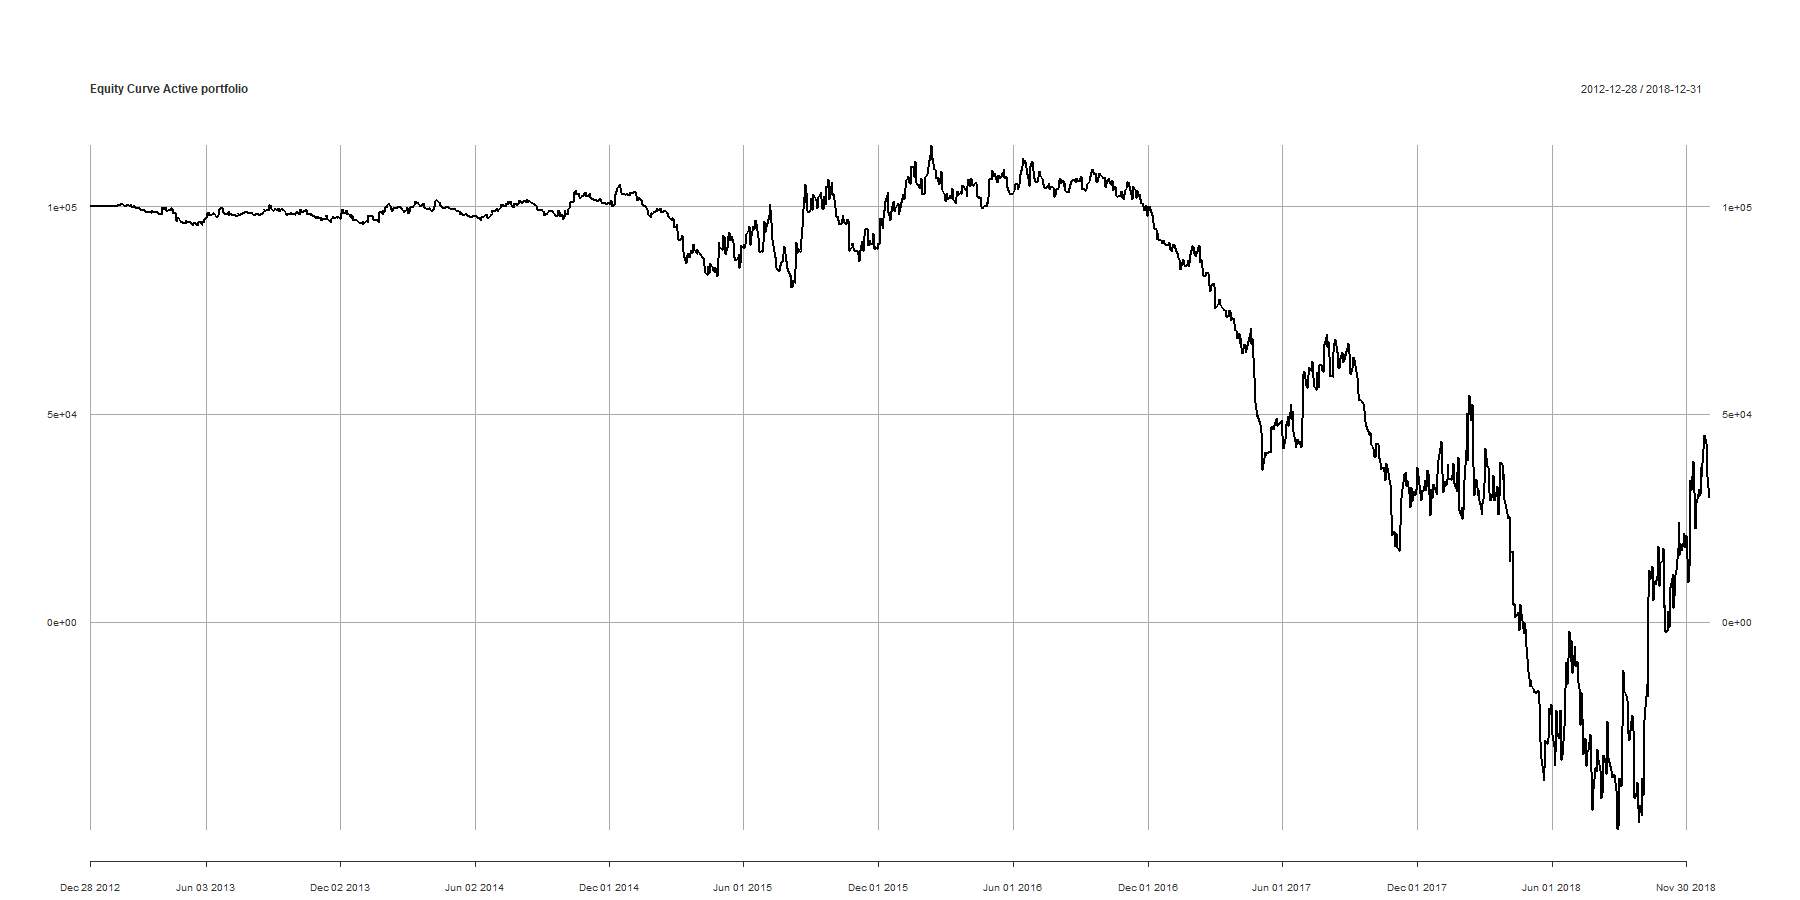
\includegraphics{"D:/2017-2018/data_analysis/technical_analysis/report/equity_active.png"}
\caption{Account Capital level at closing of active positions}
\end{figure}

\hypertarget{benchmarking-with-buy-and-hold-strategy}{%
\subsubsection{Benchmarking with buy-and-hold
strategy}\label{benchmarking-with-buy-and-hold-strategy}}

The negative performance of our active portfolio strategy prompts the
comparison with a passive strategy. We now implement a buy and hold
strategy, over the same timeframe as before, with the same stocks we
considered for our active strategy. Here we will allocate equal parts of
the initial capital to each of the five stocks, and execute a buy order
for each on the first day of observations. On the last day, we sell all
the stocks we had bought. Thus, the increase(reduction) in the stock
price will determine our gains(losses).

\begin{verbatim}
## [1] "Set capital to 100,000 Euros "
## [1] "2012-12-28 00:00:00 FP.PA 514 @ 38.91"
## [1] "2012-12-28 00:00:00 MC.PA 145 @ 137.800003"
## [1] "2012-12-28 00:00:00 SAN.PA 282 @ 70.730003"
## [1] "2012-12-28 00:00:00 AIR.PA 680 @ 29.395"
## [1] "2012-12-28 00:00:00 OR.PA 190 @ 104.800003"
## [1] "2018-12-31 00:00:00 FP.PA -514 @ 46.18"
## [1] "2018-12-31 00:00:00 MC.PA -145 @ 258.200012"
## [1] "2018-12-31 00:00:00 SAN.PA -282 @ 75.660004"
## [1] "2018-12-31 00:00:00 AIR.PA -680 @ 83.959999"
## [1] "2018-12-31 00:00:00 OR.PA -190 @ 201.199997"
\end{verbatim}

Since each stock price has risen during the five years examined, it can
be easily noted that this buy and hold strategy appears rather
profitable: our initial € 100,000 investment stake has increased by
about 80\%. At this stage, it is difficult to think that an active
strategy could have beaten the market. On the other hand, an in-depth
study is required to examine what factors determined such increases in
prices. This in turn highlights the importance of an appropriate market
study that should accompany the creation of the trading strategy.
Clearly, investing is far from gambling, and coding or mathemathical
skills cannot make up for a poor understanding of the markets.

\begin{figure}
\centering
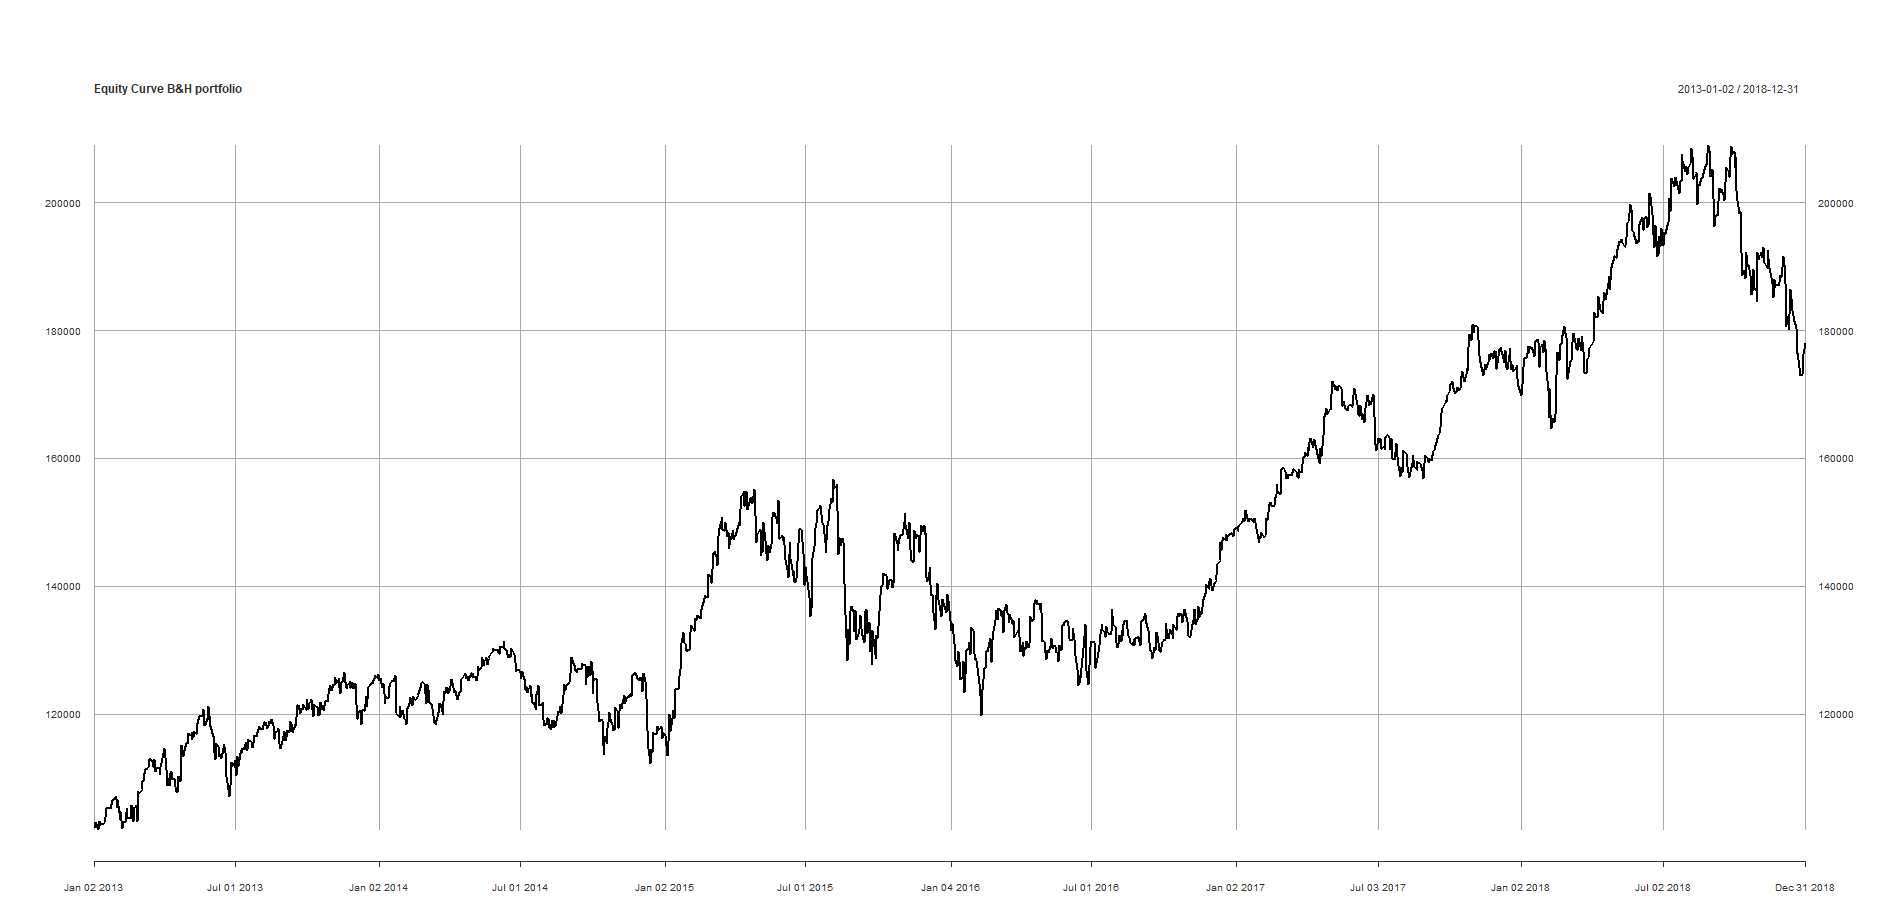
\includegraphics{"D:/2017-2018/data_analysis/technical_analysis/report/equity_BH.png"}
\caption{Account Capital level at closing of long positions in B\&H
strategy}
\end{figure}

\hypertarget{final-comments-and-future-steps}{%
\subsection{Final comments and future
steps}\label{final-comments-and-future-steps}}

It is clear that our strategy implementation lacks of several important
feautres, on which we already touched above. We left one important point
untackled - namely, the absence of a proper testing strategy. As Guy
Yollin illustrates\footnote{\url{http://www.r-programming.org/files}},
implementing a trading strategy would first require a the so-called
\emph{walk-forward analysis}, which allows for a dynamic parametrization
of the model, with a lower impact of overfitting\footnote{\url{https://algotrading101.com/learn/what-is-walk-forward-optimization/}}.
Nevertheless, we would rather highlight the importance of having created
a realistic model, which can constitute a first, solid building block
towards a proper in-depth study of TA optimized applications to trading.

\hypertarget{knitr-and-rmarkdown}{%
\subsection{knitr and Rmarkdown}\label{knitr-and-rmarkdown}}

As a final remark, we would like to add that this report was created in
Rmarkdown\footnote{\url{https://bookdown.org/yihui/rmarkdown/}} and
compiled with with \texttt{knitr}\footnote{\url{https://yihui.org/knitr/}
} .

  \bibliography{bibliography.bib}

\end{document}
